\documentclass[conference]{IEEEtran}
\usepackage{amsmath,amssymb}
\usepackage{graphicx}
\usepackage{booktabs}
\usepackage{multirow}
\usepackage{url}
\usepackage{cite}
\usepackage{color}
\usepackage{algorithm}
\usepackage{algorithmic}
\usepackage{tabularx}
\usepackage{array}
\usepackage{caption}

\begin{document}

\title{RetinaSense: An Uncertainty-Aware Domain-Adaptive Vision Transformer Framework with Retrieval-Augmented Reasoning for Multi-Disease Retinal Diagnosis}

\author{\IEEEauthorblockN{1\textsuperscript{st} Tanishq Tamarkar}
\IEEEauthorblockA{\textit{Department of Computer Science} \\
\textit{SRM Institute of Science and Technology}\\
Chennai, India \\
tanishqtam@gmail.com}
\and
\IEEEauthorblockN{2\textsuperscript{nd} Rafae Mohammed Hussain}
\IEEEauthorblockA{\textit{Department of Computer Science} \\
\textit{SRM Institute of Science and Technology}\\
Chennai, India \\
rafae@example.com}
\and
\IEEEauthorblockN{3\textsuperscript{rd} Dr. Revathi M}
\IEEEauthorblockA{\textit{Department of Computer Science} \\
\textit{SRM Institute of Science and Technology}\\
Chennai, India \\
revathi@example.com}
}
\maketitle

% ================================================================
% ABSTRACT
% ================================================================
\begin{abstract}
Early detection of retinal diseases remains essential for preventing permanent vision loss, yet most current automated screening tools handle only one disease at a time, offer limited interpretability, and tend to degrade when images come from different clinical sources. We present \textbf{RetinaSense}, an end-to-end framework for multi-disease retinal diagnosis built around a Vision Transformer (ViT-Base/16) backbone, augmented with Domain-Adversarial Neural Network (DANN) training, uncertainty estimation, and retrieval-augmented reasoning.

The framework addresses three core problems: (1) cross-dataset domain shift, handled by a Gradient Reversal Layer that pushes the backbone toward domain-invariant representations across four fundus image sources; (2) a severe 21:1 class imbalance, mitigated through focal loss with progressive class weighting and hard-example mining; and (3) the need for clinical trust, addressed through a Retrieval-Augmented Diagnosis (RAD) pipeline that combines calibrated predictions, Monte Carlo dropout uncertainty, attention-based explanations, and FAISS-based similar case retrieval.

We trained the system on 11,524 fundus images drawn from APTOS, ODIR, REFUGE2, and MESSIDOR-2. On a held-out test set spanning five conditions---Normal, Diabetic Retinopathy, Glaucoma, Cataract, and Age-related Macular Degeneration---RetinaSense reaches \textbf{89.30\%} accuracy, \textbf{0.886 macro F1-score}, and \textbf{0.975 macro AUC}, representing a $+3.8\%$ absolute accuracy gain over the base ViT without domain adaptation in our ablation study. Temperature scaling brings the Expected Calibration Error down to 0.034. The FAISS retrieval component scores 0.921 Mean Average Precision with 94.0\% class-match recall at $K\!=\!1$, pushing combined accuracy to 94.0\% ($+4.9\%$). A confidence routing mechanism auto-reports 76.9\% of cases at 96.8\% accuracy and catches 77.2\% of errors before they reach clinicians. Taken together, these results suggest that pairing domain adaptation with uncertainty estimation and retrieval can meaningfully improve both the accuracy and the clinical utility of automated retinal screening.
\end{abstract}

\begin{IEEEkeywords}
Retinal disease classification, Vision Transformer, domain adaptation, DANN, uncertainty estimation, retrieval-augmented diagnosis, fundus image analysis, class imbalance
\end{IEEEkeywords}

% ================================================================
% I. INTRODUCTION
% ================================================================
\section{Introduction}

Diabetic Retinopathy (DR), Glaucoma, Cataract, and Age-related Macular Degeneration (AMD) rank among the leading causes of preventable blindness worldwide, collectively affecting more than 500 million people \cite{b1,b27}. Fundus photography enables early detection that can guide timely treatment, but there simply are not enough trained ophthalmologists to meet the demand---especially in low-resource settings \cite{b2}.

Deep learning has shown considerable promise for retinal image analysis \cite{b3,b4}, yet moving these models into clinical practice brings up several persistent challenges. Most published systems target a \textit{single disease}, which limits their usefulness in a clinic where patients may present with any of several conditions. Models trained on one dataset frequently underperform on images from a different hospital or camera---a phenomenon called \textit{domain shift}---because differences in imaging hardware, preprocessing pipelines, and patient demographics change the image distribution in ways that confuse the classifier. On top of that, rare conditions like AMD may represent as little as 3\% of the data, so \textit{class imbalance} biases models toward the majority classes. And without \textit{uncertainty quantification} or \textit{evidence-based reasoning}, clinicians have little basis for trusting the system's outputs.

We set out to address these gaps with \textbf{RetinaSense}, a framework that goes beyond standard classification by bringing together:

\begin{itemize}
    \item A \textbf{Domain-Adversarial Neural Network (DANN)} with a Gradient Reversal Layer \cite{b13} that learns features shared across four different fundus image sources. In our experiments, this brought APTOS domain accuracy from 26.5\% up to 100\%.
    \item A \textbf{multi-strategy training pipeline} that pairs focal loss with progressive class weighting, hard-example mining, mixup augmentation, and cosine annealing---all aimed at a 21:1 class imbalance.
    \item A \textbf{Retrieval-Augmented Diagnosis (RAD)} pipeline that ties together temperature-calibrated predictions (ECE=0.034), Monte Carlo dropout uncertainty \cite{b7}, attention-based explainability, and FAISS-based similar case retrieval \cite{b9} into a single clinical decision-support workflow.
    \item A \textbf{confidence routing} mechanism that sorts predictions into auto-report, review, or escalation categories based on model confidence, MC Dropout uncertainty, and retrieval agreement.
\end{itemize}

In summary, our contributions are:
\begin{enumerate}
    \item A domain-adversarial ViT architecture that achieves 89.30\% accuracy on multi-source, multi-disease retinal classification with 0.975 macro AUC.
    \item A progressive training strategy combining eight complementary techniques to handle simultaneous domain shift and class imbalance.
    \item A Retrieval-Augmented Diagnosis pipeline that grounds predictions in evidence---calibrated uncertainty and retrieved similar cases---for clinical trustworthiness.
    \item A thorough evaluation across four datasets, including ablation studies, calibration analysis, and detailed error characterization.
\end{enumerate}

% ================================================================
% II. RELATED WORK
% ================================================================
\section{Related Work}

\subsection{Deep Learning for Retinal Disease Detection}

The landmark study by Gulshan \textit{et al.} \cite{b3} showed that deep CNNs could match ophthalmologist-level sensitivity for DR detection, and the Kaggle diabetic retinopathy competitions \cite{b29} spurred rapid progress in the years that followed. Architectures like EfficientNet \cite{b5} and ResNet \cite{b6} have since become standard architectures for fundus analysis, with transfer learning from ImageNet making it feasible to train on relatively small medical datasets. That said, the bulk of this work still centers on binary or single-disease classification, which falls short of what a real screening program needs.

\subsection{Vision Transformers in Medical Imaging}

Dosovitskiy \textit{et al.} \cite{b8} introduced the Vision Transformer (ViT), which splits an image into patches and runs them through transformer encoder blocks with multi-head self-attention. One practical advantage over CNNs is that ViT has a global receptive field from the very first layer. Touvron \textit{et al.} \cite{b28} later improved training efficiency with data-efficient transformers and knowledge distillation. In the medical domain, Zhou \textit{et al.} \cite{b14} and Chen \textit{et al.} \cite{b15} have applied transformers with encouraging results, though we are not aware of a systematic study that evaluates multi-class retinal classification under severe imbalance.

\subsection{Domain Adaptation in Medical Imaging}

When datasets from different institutions or cameras are combined, domain shift is nearly unavoidable. Ganin \textit{et al.} \cite{b13} proposed the Domain-Adversarial Neural Network (DANN), where a Gradient Reversal Layer (GRL) forces the feature extractor to learn representations that a domain discriminator cannot distinguish---in effect, stripping away source-specific artifacts. DANN has been adopted in medical imaging \cite{b16}, but to our knowledge it has not been combined with a Vision Transformer backbone for multi-source retinal classification.

\subsection{Uncertainty Estimation and Retrieval-Augmented Systems}

Gal and Ghahramani \cite{b7} showed that MC Dropout can serve as a practical Bayesian approximation for uncertainty. On a separate front, FAISS \cite{b9} makes large-scale similarity search fast enough for real-time case-based reasoning. What is missing in the literature is a system that ties domain adaptation, calibrated uncertainty, and visual evidence retrieval together in one retinal screening pipeline. That is the gap we aim to fill.

% ================================================================
% III. METHODOLOGY
% ================================================================
\section{Methodology}

\subsection{Overview of the Proposed Framework}

At a high level, RetinaSense processes each fundus image through five stages:

\begin{equation*}
\text{Input} \!\rightarrow\! \text{CLAHE} \!\rightarrow\! \text{DANN-ViT} \!\rightarrow\! \text{Calibrate} \!\rightarrow\! \text{RAD} \!\rightarrow\! \text{Output}
\end{equation*}

\noindent The RAD step encompasses uncertainty estimation, retrieval, and confidence routing. Fig.~\ref{fig:architecture} shows the full system architecture.

\begin{figure*}[t]
\centering
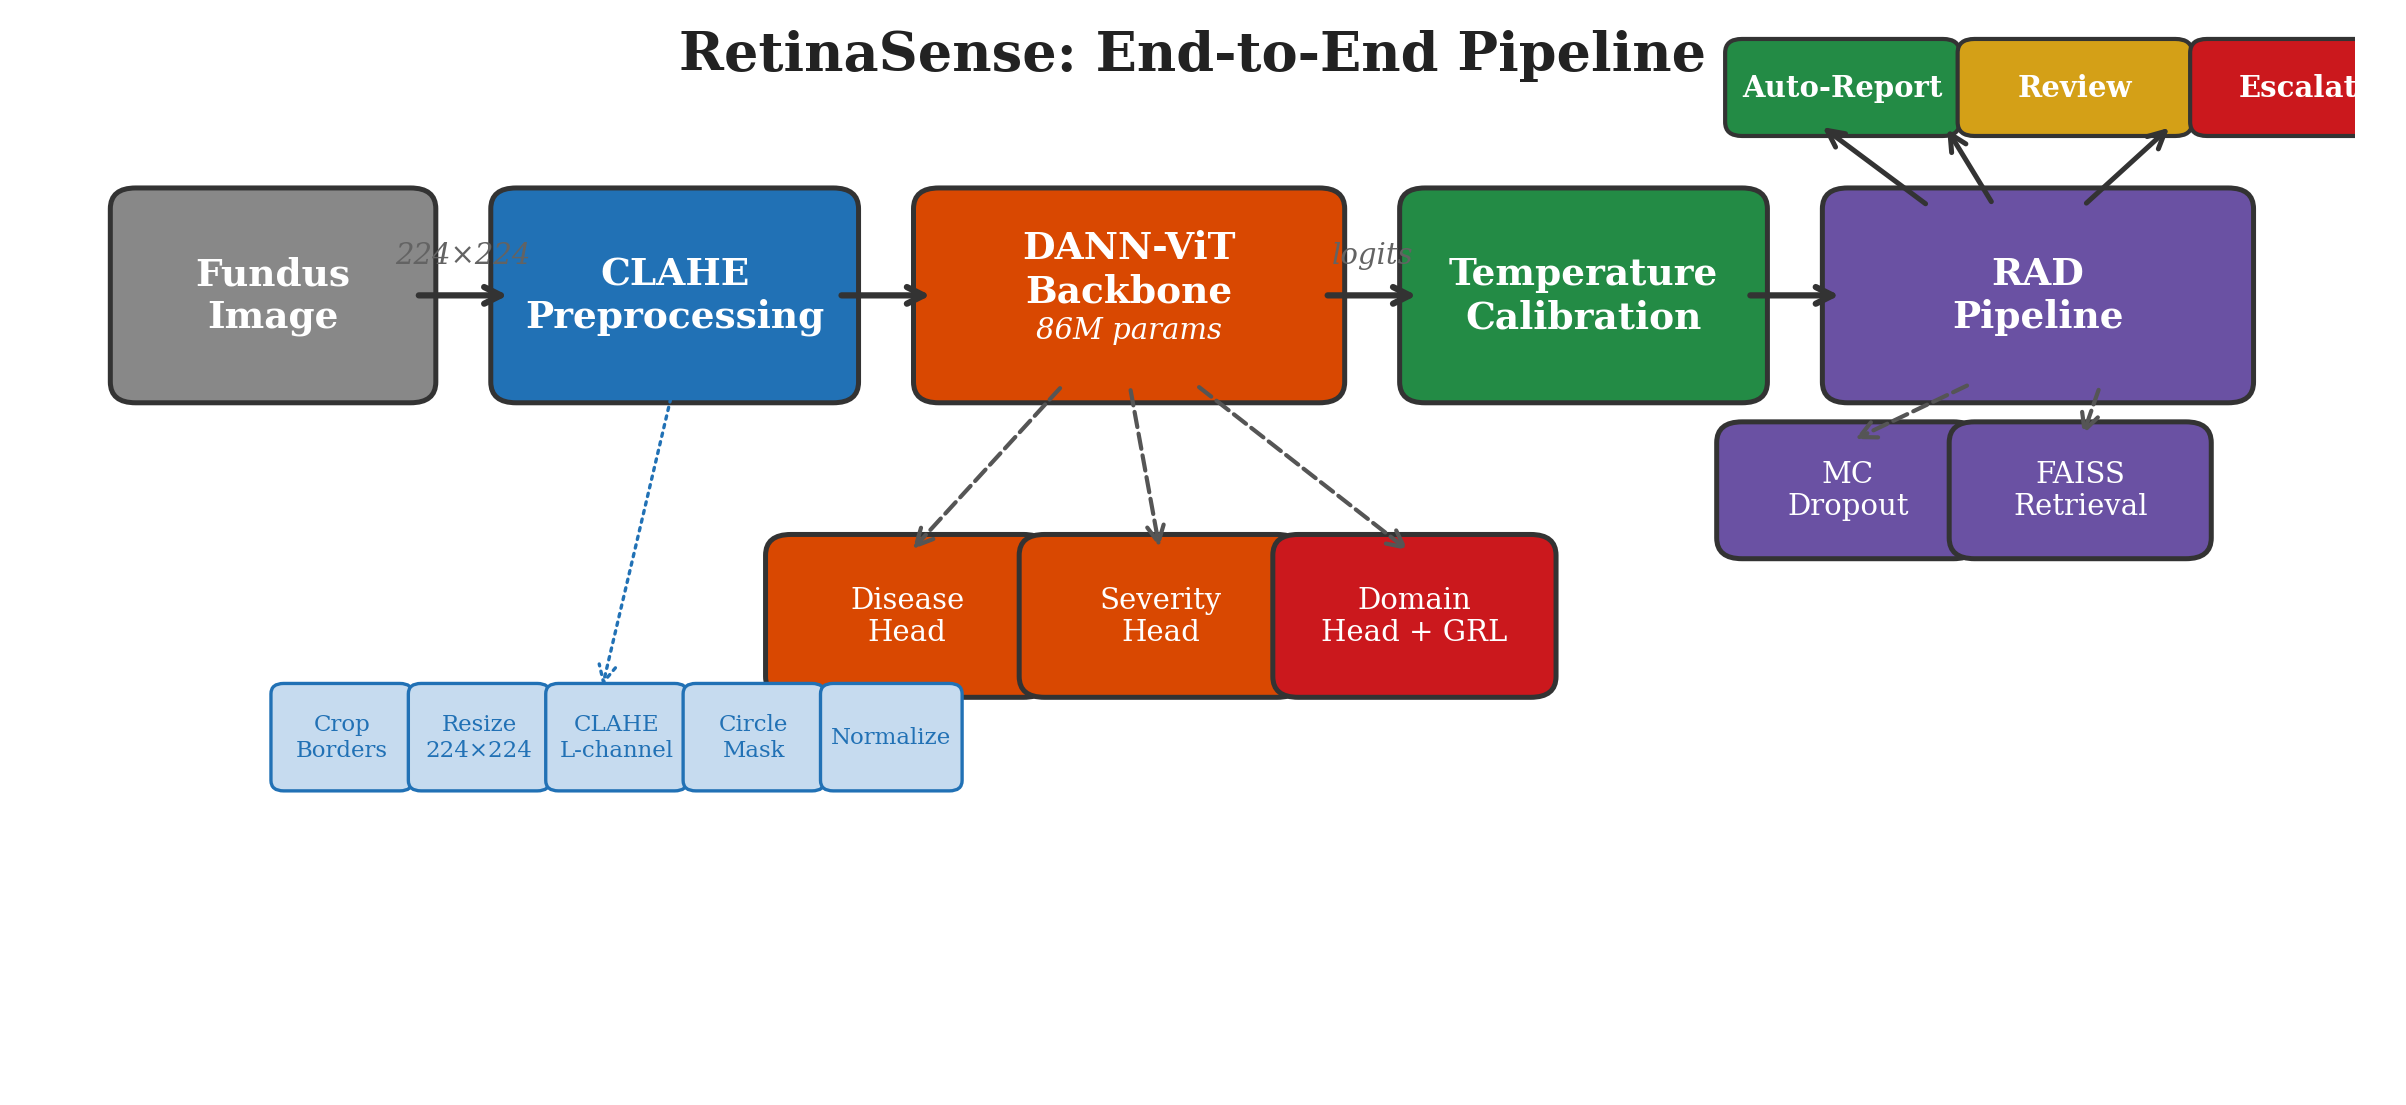
\includegraphics[width=0.95\textwidth]{figures/fig_system_architecture.png}
\caption{RetinaSense end-to-end pipeline. Fundus images undergo CLAHE preprocessing, are classified by the DANN-ViT backbone (with disease, severity, and domain heads), calibrated via temperature scaling, and processed through the RAD pipeline for uncertainty estimation, retrieval, and confidence-based clinical routing.}
\label{fig:architecture}
\end{figure*}

\subsection{Image Preprocessing}

Every image---regardless of which dataset it comes from---passes through the same Contrast-Limited Adaptive Histogram Equalization (CLAHE) pipeline. This is deliberate: by standardizing preprocessing we avoid introducing domain shift at the input stage.

\begin{enumerate}
    \item Black border cropping via thresholding
    \item Resizing to $224 \times 224$ pixels
    \item CLAHE on the L-channel (clipLimit=2.0, tileGrid=$8\times8$)
    \item Circular masking (radius = $0.48 \times$ image size)
    \item Normalization with dataset-specific statistics ($\mu=[0.590, 0.446, 0.334]$, $\sigma=[0.165, 0.157, 0.178]$)
\end{enumerate}

\subsection{DANN Architecture}

The backbone is a ViT-Base/16 \cite{b8,b30} with 86M parameters, producing a 768-dimensional CLS token. Three task-specific heads branch off from this shared representation:

\textbf{Disease Classification Head:}
\begin{equation}
H_d: \mathbb{R}^{768} \rightarrow \mathbb{R}^{512} \rightarrow \mathbb{R}^{256} \rightarrow \mathbb{R}^{5}
\end{equation}
with BatchNorm, ReLU, and Dropout (0.3, 0.2) between layers.

\textbf{Severity Grading Head:}
\begin{equation}
H_s: \mathbb{R}^{768} \rightarrow \mathbb{R}^{256} \rightarrow \mathbb{R}^{5}
\end{equation}

\textbf{Domain Discriminator Head} (preceded by a Gradient Reversal Layer):
\begin{equation}
H_{dom}: \text{GRL}_\lambda(f) \rightarrow \mathbb{R}^{256} \rightarrow \mathbb{R}^{64} \rightarrow \mathbb{R}^{4}
\end{equation}

During the forward pass the GRL acts as an identity, but during backpropagation it flips the sign of the gradients. This forces the backbone to learn features that the domain discriminator \textit{cannot} use to distinguish between sources:
\begin{equation}
\text{GRL}_\lambda(x) = x \quad (\text{forward}), \quad \frac{\partial \text{GRL}}{\partial x} = -\lambda I \quad (\text{backward})
\end{equation}

We schedule the adversarial strength $\lambda$ using the Ganin schedule \cite{b13}, with a cap at 0.3:
\begin{equation}
\lambda_p = \min\!\left(\frac{2}{1 + e^{-10p}} - 1,\; 0.3\right), \quad p = \frac{\text{epoch}}{T}
\end{equation}

\noindent Fig.~\ref{fig:dann_arch} illustrates the full DANN-ViT architecture.

\begin{figure}[h]
\centering
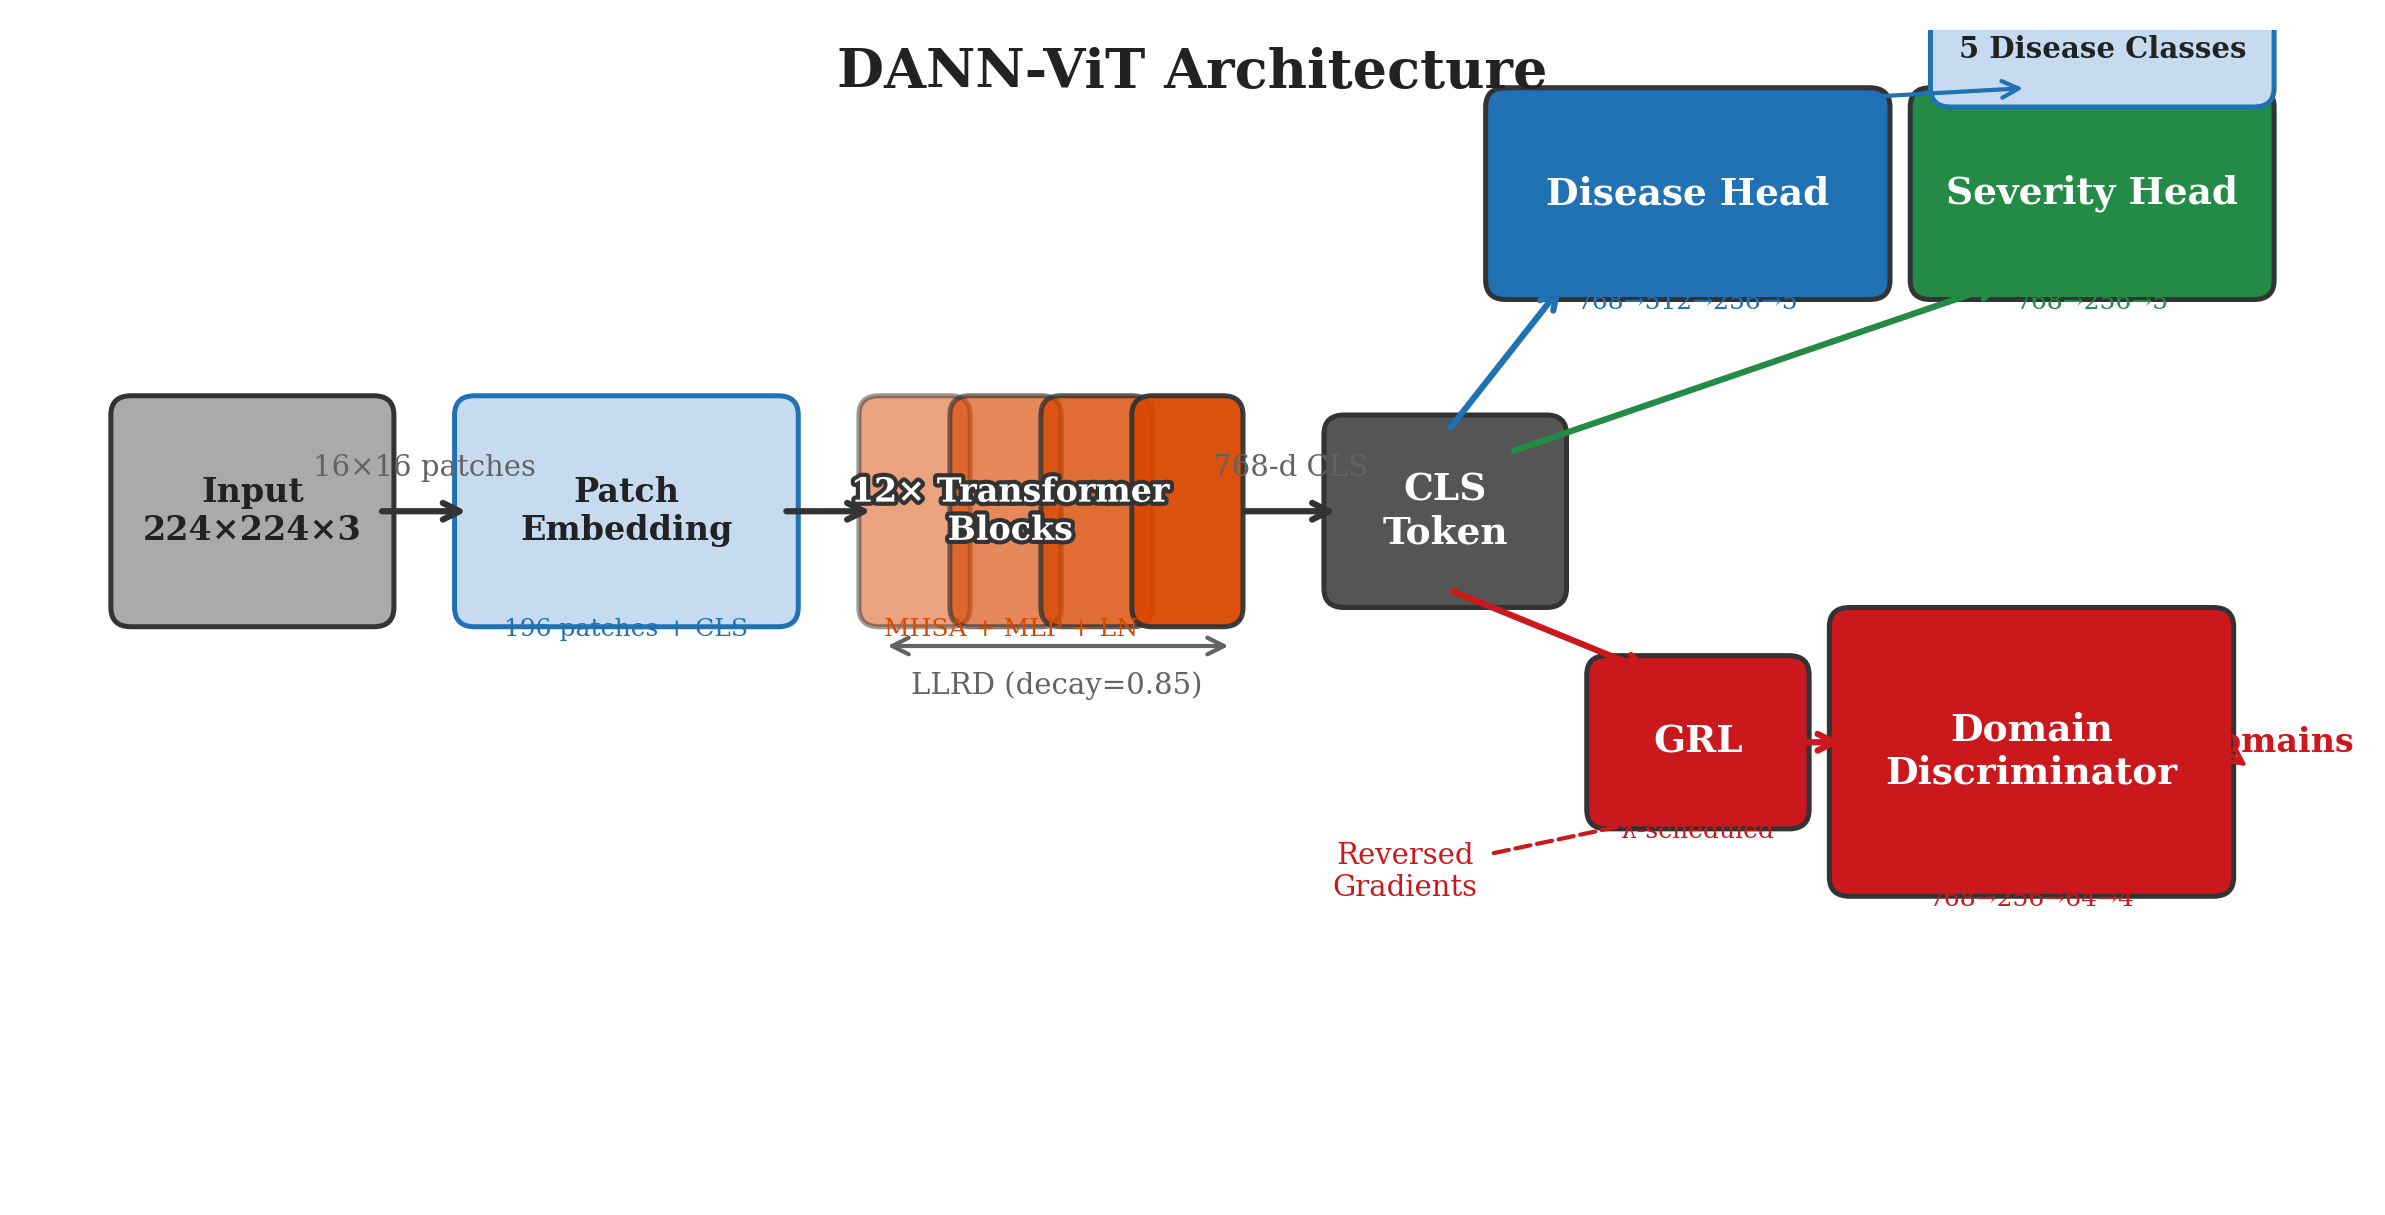
\includegraphics[width=0.95\linewidth]{figures/fig_dann_architecture.png}
\caption{DANN-ViT architecture. The ViT-Base/16 backbone extracts a 768-d CLS token, which feeds three heads: disease classification (5 classes), severity grading (5 levels), and domain discrimination (4 sources) with a Gradient Reversal Layer (GRL). LLRD applies decaying learning rates across the 12 transformer blocks.}
\label{fig:dann_arch}
\end{figure}

\subsection{Training Strategy}

Training optimizes a combined loss over disease classification, severity grading, and domain discrimination:
\begin{equation}
\mathcal{L} = \mathcal{L}_{disease} + 0.2 \cdot \mathcal{L}_{severity} + w_{dom} \cdot \lambda_p \cdot \mathcal{L}_{domain}
\end{equation}

Because our data suffers from both domain shift and class imbalance, we found it necessary to combine several complementary strategies rather than relying on any single fix:

\begin{enumerate}
    \item \textbf{Focal Loss} \cite{b12} with per-class weights: $\mathcal{L}_{focal} = -\alpha_c(1-p_t)^\gamma \log(p_t)$, $\gamma=2.0$
    \item \textbf{Progressive DR Alpha Boost}: The class weight for DR ramps linearly from $1.5\times$ to $3.0\times$ over the course of training
    \item \textbf{Hard-Example Mining}: Each epoch, the 500 samples with the highest loss are oversampled $2\times$; DR$\rightarrow$Normal misclassifications get an extra boost
    \item \textbf{Class-Balanced Sampling}: A WeightedRandomSampler with inverse-frequency weights
    \item \textbf{Mixup Augmentation} \cite{b11}: $\alpha=0.2$, applied to half the batches (disease labels only---we leave domain labels untouched)
    \item \textbf{Label Smoothing}: Factor of 0.1 on the disease loss
    \item \textbf{Cosine Annealing with Warm Restarts}: $T_0=10$, $T_{mult}=2$
    \item \textbf{Layer-wise Learning Rate Decay (LLRD)}: Decay factor 0.85 across the 12 transformer blocks
\end{enumerate}

\noindent We use AdamW \cite{b25} with a base learning rate of $3\times10^{-5}$, weight decay $10^{-4}$, gradient accumulation to reach an effective batch size of 128, and AMP mixed precision throughout.

\subsection{Calibration and Threshold Optimization}

After training, we apply temperature scaling on the calibration set:
\begin{equation}
p_i = \text{softmax}(z_i / T), \quad T^* = \arg\min_T \text{NLL}(T)
\end{equation}

We also optimize per-class decision thresholds via grid search on the calibration set, targeting per-class F1-score. This turns out to be especially helpful for the minority classes.

\subsection{Retrieval-Augmented Diagnosis (RAD) Pipeline}

The RAD pipeline is designed to give clinicians more than just a label. It has four components:

\textbf{1) Uncertainty Estimation:} We run $T=15$ stochastic forward passes with MC Dropout and decompose the resulting uncertainty into:
\begin{itemize}
    \item Predictive entropy: $H[\bar{p}] = -\sum_c \bar{p}_c \log \bar{p}_c$ (total uncertainty)
    \item Expected entropy: $\mathbb{E}[H[p_t]]$ (aleatoric/data uncertainty)
    \item Mutual information: $H[\bar{p}] - \mathbb{E}[H[p_t]]$ (epistemic/model uncertainty)
\end{itemize}

\textbf{2) Visual Evidence Retrieval:} We build a FAISS index over L2-normalized 768-dim ViT embeddings for every training sample. At inference time, we retrieve the top-$K$ nearest neighbors by inner product (which amounts to cosine similarity after normalization).

\textbf{3) Retrieval-Augmented Prediction:} The class distribution from the retrieved neighbors is blended with the model's own prediction:
\begin{equation}
p_{final} = \alpha \cdot p_{model} + (1-\alpha) \cdot p_{kNN}
\end{equation}
where $\alpha=0.85$ by default. We also compute an \textit{agreement score} that measures how well the retrieved cases support the model's top prediction.

\textbf{4) Confidence Routing:} Based on the combined signals, each prediction is placed into one of three clinical tiers:
\begin{itemize}
    \item \textbf{Auto-Report}: High confidence ($>0.85$), low entropy ($<0.5$), and retrieval agreement
    \item \textbf{Review}: Moderate confidence, or the retrieved cases disagree with the model
    \item \textbf{Escalate}: Low confidence ($<0.5$), high entropy ($>1.0$), or flagged as out-of-distribution
\end{itemize}

\noindent Fig.~\ref{fig:rad_pipeline} shows the complete RAD pipeline.

\begin{figure}[h]
\centering
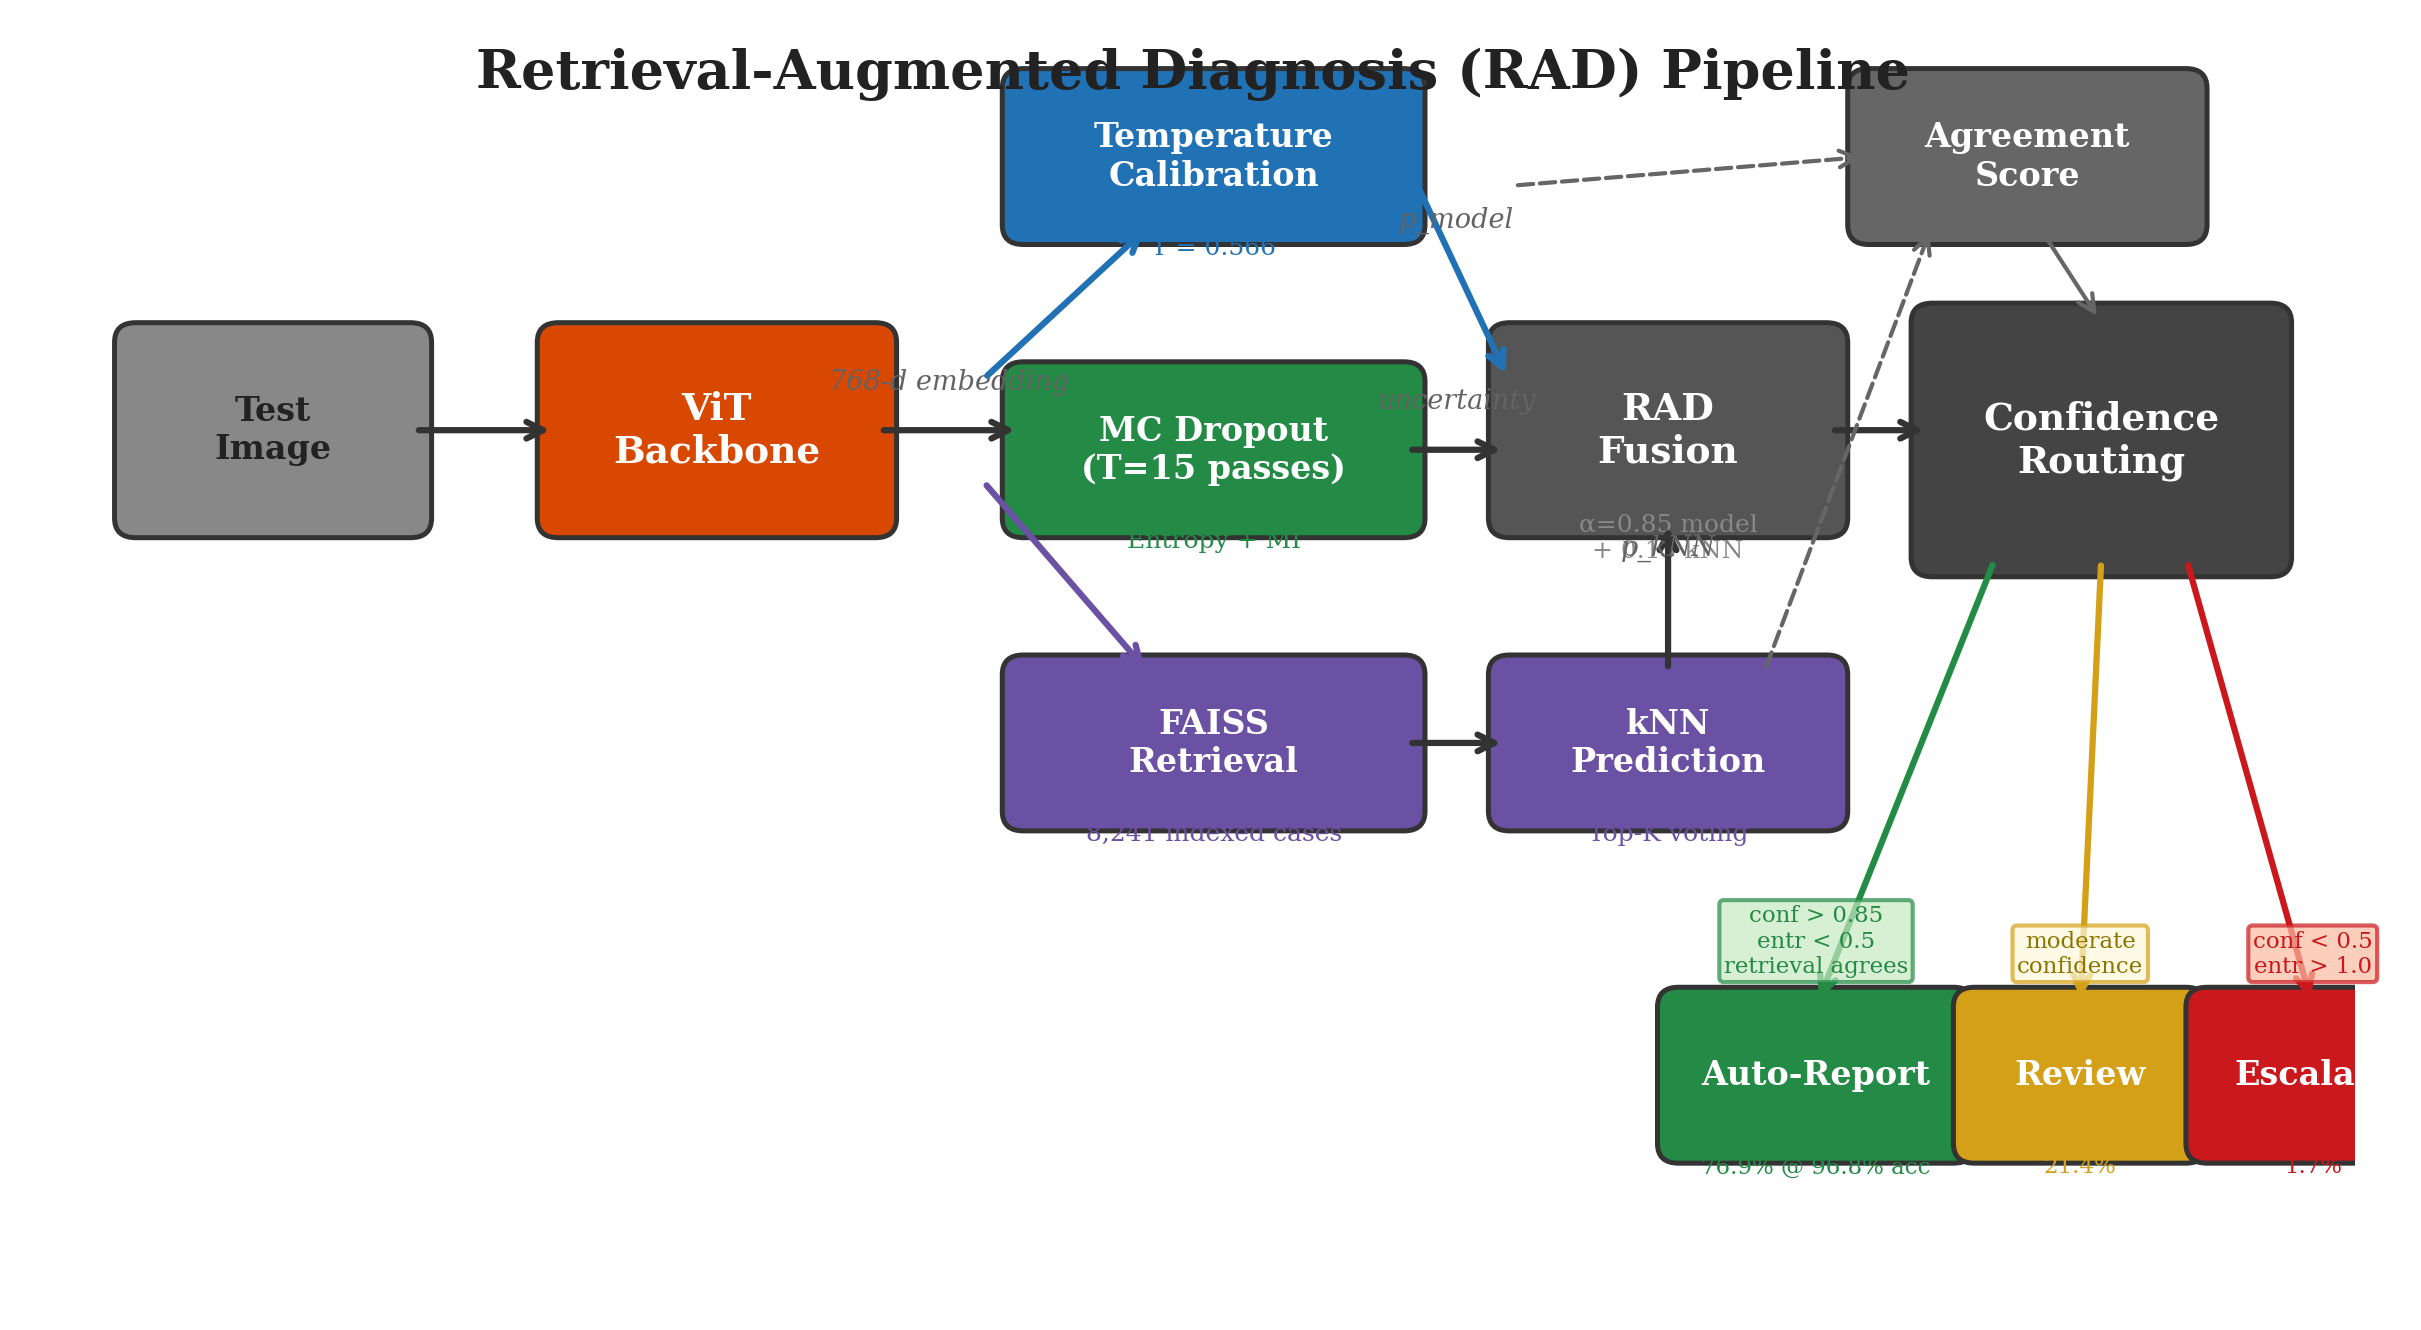
\includegraphics[width=0.95\linewidth]{figures/fig_rad_pipeline.png}
\caption{Retrieval-Augmented Diagnosis (RAD) pipeline. A test image embedding is processed through three parallel branches---temperature calibration, MC Dropout uncertainty, and FAISS retrieval---then fused and routed to Auto-Report (76.9\% at 96.8\% accuracy), Review, or Escalate tiers.}
\label{fig:rad_pipeline}
\end{figure}

\subsection{Explainability}

For visual explanations we use Attention Rollout \cite{b17} rather than the more common Grad-CAM \cite{b10}. The reason is practical: standard Grad-CAM produces zero gradients for ViT patch tokens due to the CLS token bottleneck. Rollout sidesteps this by recursively multiplying the attention matrices across all 12 transformer layers, yielding a spatial attention map over the $14\times14$ patch grid.

% ================================================================
% IV. DATASET
% ================================================================
\section{Dataset}

\subsection{Data Sources}

We assembled a composite dataset of 11,524 fundus images from four public sources, summarized in Table~\ref{tab:dataset_sources}. Each source contributes a different subset of disease classes and comes with its own imaging characteristics, which is precisely what makes domain adaptation necessary.

\begin{table}[h]
\centering
\caption{Dataset Composition by Source}
\label{tab:dataset_sources}
\begin{tabular}{lrrr}
\toprule
\textbf{Source} & \textbf{Images} & \textbf{Classes} & \textbf{Domain} \\
\midrule
APTOS-2019 \cite{b19} & 3,662 & DR only & 0 \\
ODIR-5K \cite{b18} & 4,878 & All 5 & 1 \\
REFUGE2 \cite{b20} & 1,240 & Nor+Glau & 2 \\
MESSIDOR-2 \cite{b21} & 1,744 & Nor+DR & 3 \\
\midrule
\textbf{Total} & \textbf{11,524} & & \\
\bottomrule
\end{tabular}
\end{table}

\subsection{Class Distribution and Imbalance}

The class distribution is heavily skewed, with a 21:1 ratio between the most and least represented classes:

\begin{table}[h]
\centering
\caption{Class Distribution Across Splits}
\label{tab:class_dist}
\begin{tabular}{lrrrrr}
\toprule
\textbf{Split} & \textbf{Nor} & \textbf{DR} & \textbf{Glau} & \textbf{Cat} & \textbf{AMD} \\
\midrule
Train (71.5\%) & 3,075 & 4,489 & 272 & 220 & 185 \\
Calib (15.8\%) & 689 & 982 & 58 & 47 & 40 \\
Test (12.7\%) & 484 & 837 & 58 & 48 & 40 \\
\midrule
\textbf{Total} & \textbf{4,248} & \textbf{6,308} & \textbf{388} & \textbf{315} & \textbf{265} \\
\bottomrule
\end{tabular}
\end{table}

\noindent Glaucoma, Cataract, and AMD together make up just 8.4\% of the dataset, which makes this a genuinely challenging multi-class imbalanced classification problem \cite{b26}. Fig.~\ref{fig:class_dist} visualizes the split.

\begin{figure}[h]
\centering
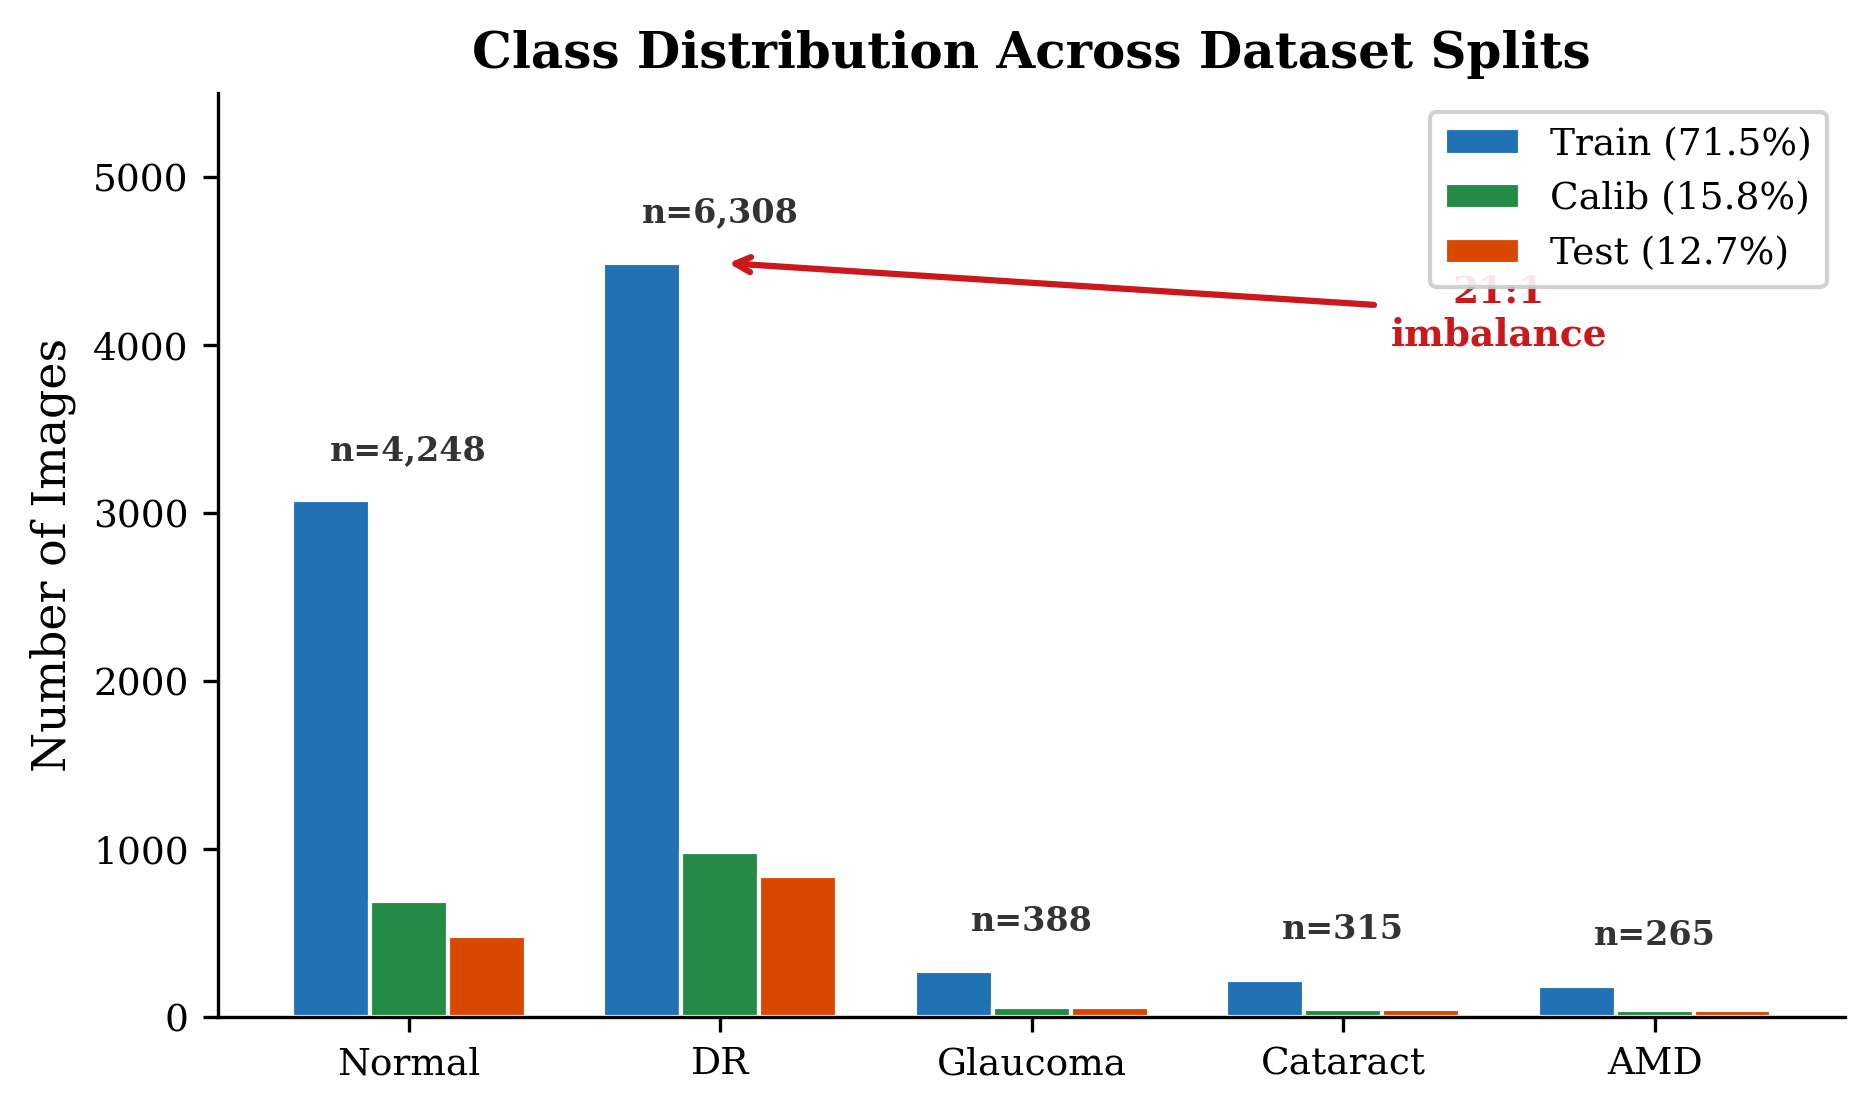
\includegraphics[width=0.95\linewidth]{figures/fig_class_distribution.png}
\caption{Class distribution across train, calibration, and test splits. DR dominates with 6,308 images (54.7\%) while AMD has only 265 (2.3\%), creating a 21:1 class imbalance ratio.}
\label{fig:class_dist}
\end{figure}

% ================================================================
% V. EXPERIMENTAL SETUP
% ================================================================
\section{Experimental Setup}

\subsection{Training Configuration}

Table~\ref{tab:hyperparams} lists the key hyperparameters. Training ran on a single NVIDIA H100 GPU and finished in under 6 minutes.

\begin{table}[h]
\centering
\caption{Training Hyperparameters}
\label{tab:hyperparams}
\begin{tabular}{ll}
\toprule
\textbf{Parameter} & \textbf{Value} \\
\midrule
Backbone & ViT-Base/16 (ImageNet-21k) \\
Parameters & 86M \\
Optimizer & AdamW (LLRD, decay=0.85) \\
Base Learning Rate & $3 \times 10^{-5}$ \\
Effective Batch Size & 128 (64 $\times$ 2 grad accum) \\
Epochs & 40 (early stopped at 31) \\
Patience & 15 (on macro F1) \\
Focal Loss $\gamma$ & 2.0 \\
Domain Weight & 0.05 \\
Label Smoothing & 0.1 \\
Mixup $\alpha$ & 0.2 (prob=0.5) \\
Hardware & NVIDIA H100 80GB \\
Training Time & 5.9 minutes \\
\bottomrule
\end{tabular}
\end{table}

\subsection{Warm-Starting Strategy}

Rather than training from scratch, we warm-start DANN-v3 from a DANN-v2 checkpoint that had already reached 86.1\% accuracy on 3 domains. Parameters with matching shapes are transferred directly; the domain discriminator head is re-initialized since it now needs to distinguish 4 sources instead of 3 (MESSIDOR-2 was added).

\subsection{Evaluation Metrics}

We report accuracy, macro F1-score, weighted F1-score, macro AUC-ROC, Cohen's kappa, Matthews Correlation Coefficient (MCC), and Expected Calibration Error (ECE). All metrics come from the sealed test set ($n=1{,}467$), which was never used during training or threshold optimization.

% ================================================================
% VI. RESULTS AND EVALUATION
% ================================================================
\section{Results and Evaluation}

\subsection{Overall Classification Performance}

Table~\ref{tab:overall_results} summarizes the test set results.

\begin{table}[h]
\centering
\caption{Overall Test Set Performance (DANN-v3)}
\label{tab:overall_results}
\begin{tabular}{lr}
\toprule
\textbf{Metric} & \textbf{Value} \\
\midrule
Overall Accuracy & \textbf{89.30\%} \\
Macro F1-Score & \textbf{0.886} \\
Weighted F1-Score & 0.893 \\
Macro AUC-ROC & \textbf{0.975} \\
Cohen's Kappa & 0.809 \\
Matthews Correlation & 0.810 \\
ECE (calibrated) & \textbf{0.034} \\
Temperature $T$ & 0.566 \\
\bottomrule
\end{tabular}
\end{table}

\subsection{Per-Class Performance}

\begin{table}[h]
\centering
\caption{Per-Class Performance on Test Set}
\label{tab:perclass}
\begin{tabular}{lccccc}
\toprule
\textbf{Class} & \textbf{Prec} & \textbf{Rec} & \textbf{F1} & \textbf{AUC} & \textbf{$n$} \\
\midrule
Normal & 0.817 & 0.895 & 0.854 & 0.964 & 484 \\
DR & 0.935 & 0.904 & 0.920 & 0.977 & 837 \\
Glaucoma & 0.900 & 0.776 & 0.833 & 0.953 & 58 \\
Cataract & 0.976 & 0.833 & 0.899 & 0.985 & 48 \\
AMD & 0.944 & 0.850 & 0.895 & 0.995 & 40 \\
\bottomrule
\end{tabular}
\end{table}

\noindent Every class achieves AUC above 0.95, with AMD reaching 0.995. What stands out is that the three minority classes---Glaucoma, Cataract, and AMD---post F1 scores between 0.833 and 0.899 despite having only 40 to 58 test samples each, which speaks to the effectiveness of the class-balancing strategy. Fig.~\ref{fig:roc} shows the per-class ROC curves.

\begin{figure}[h]
\centering
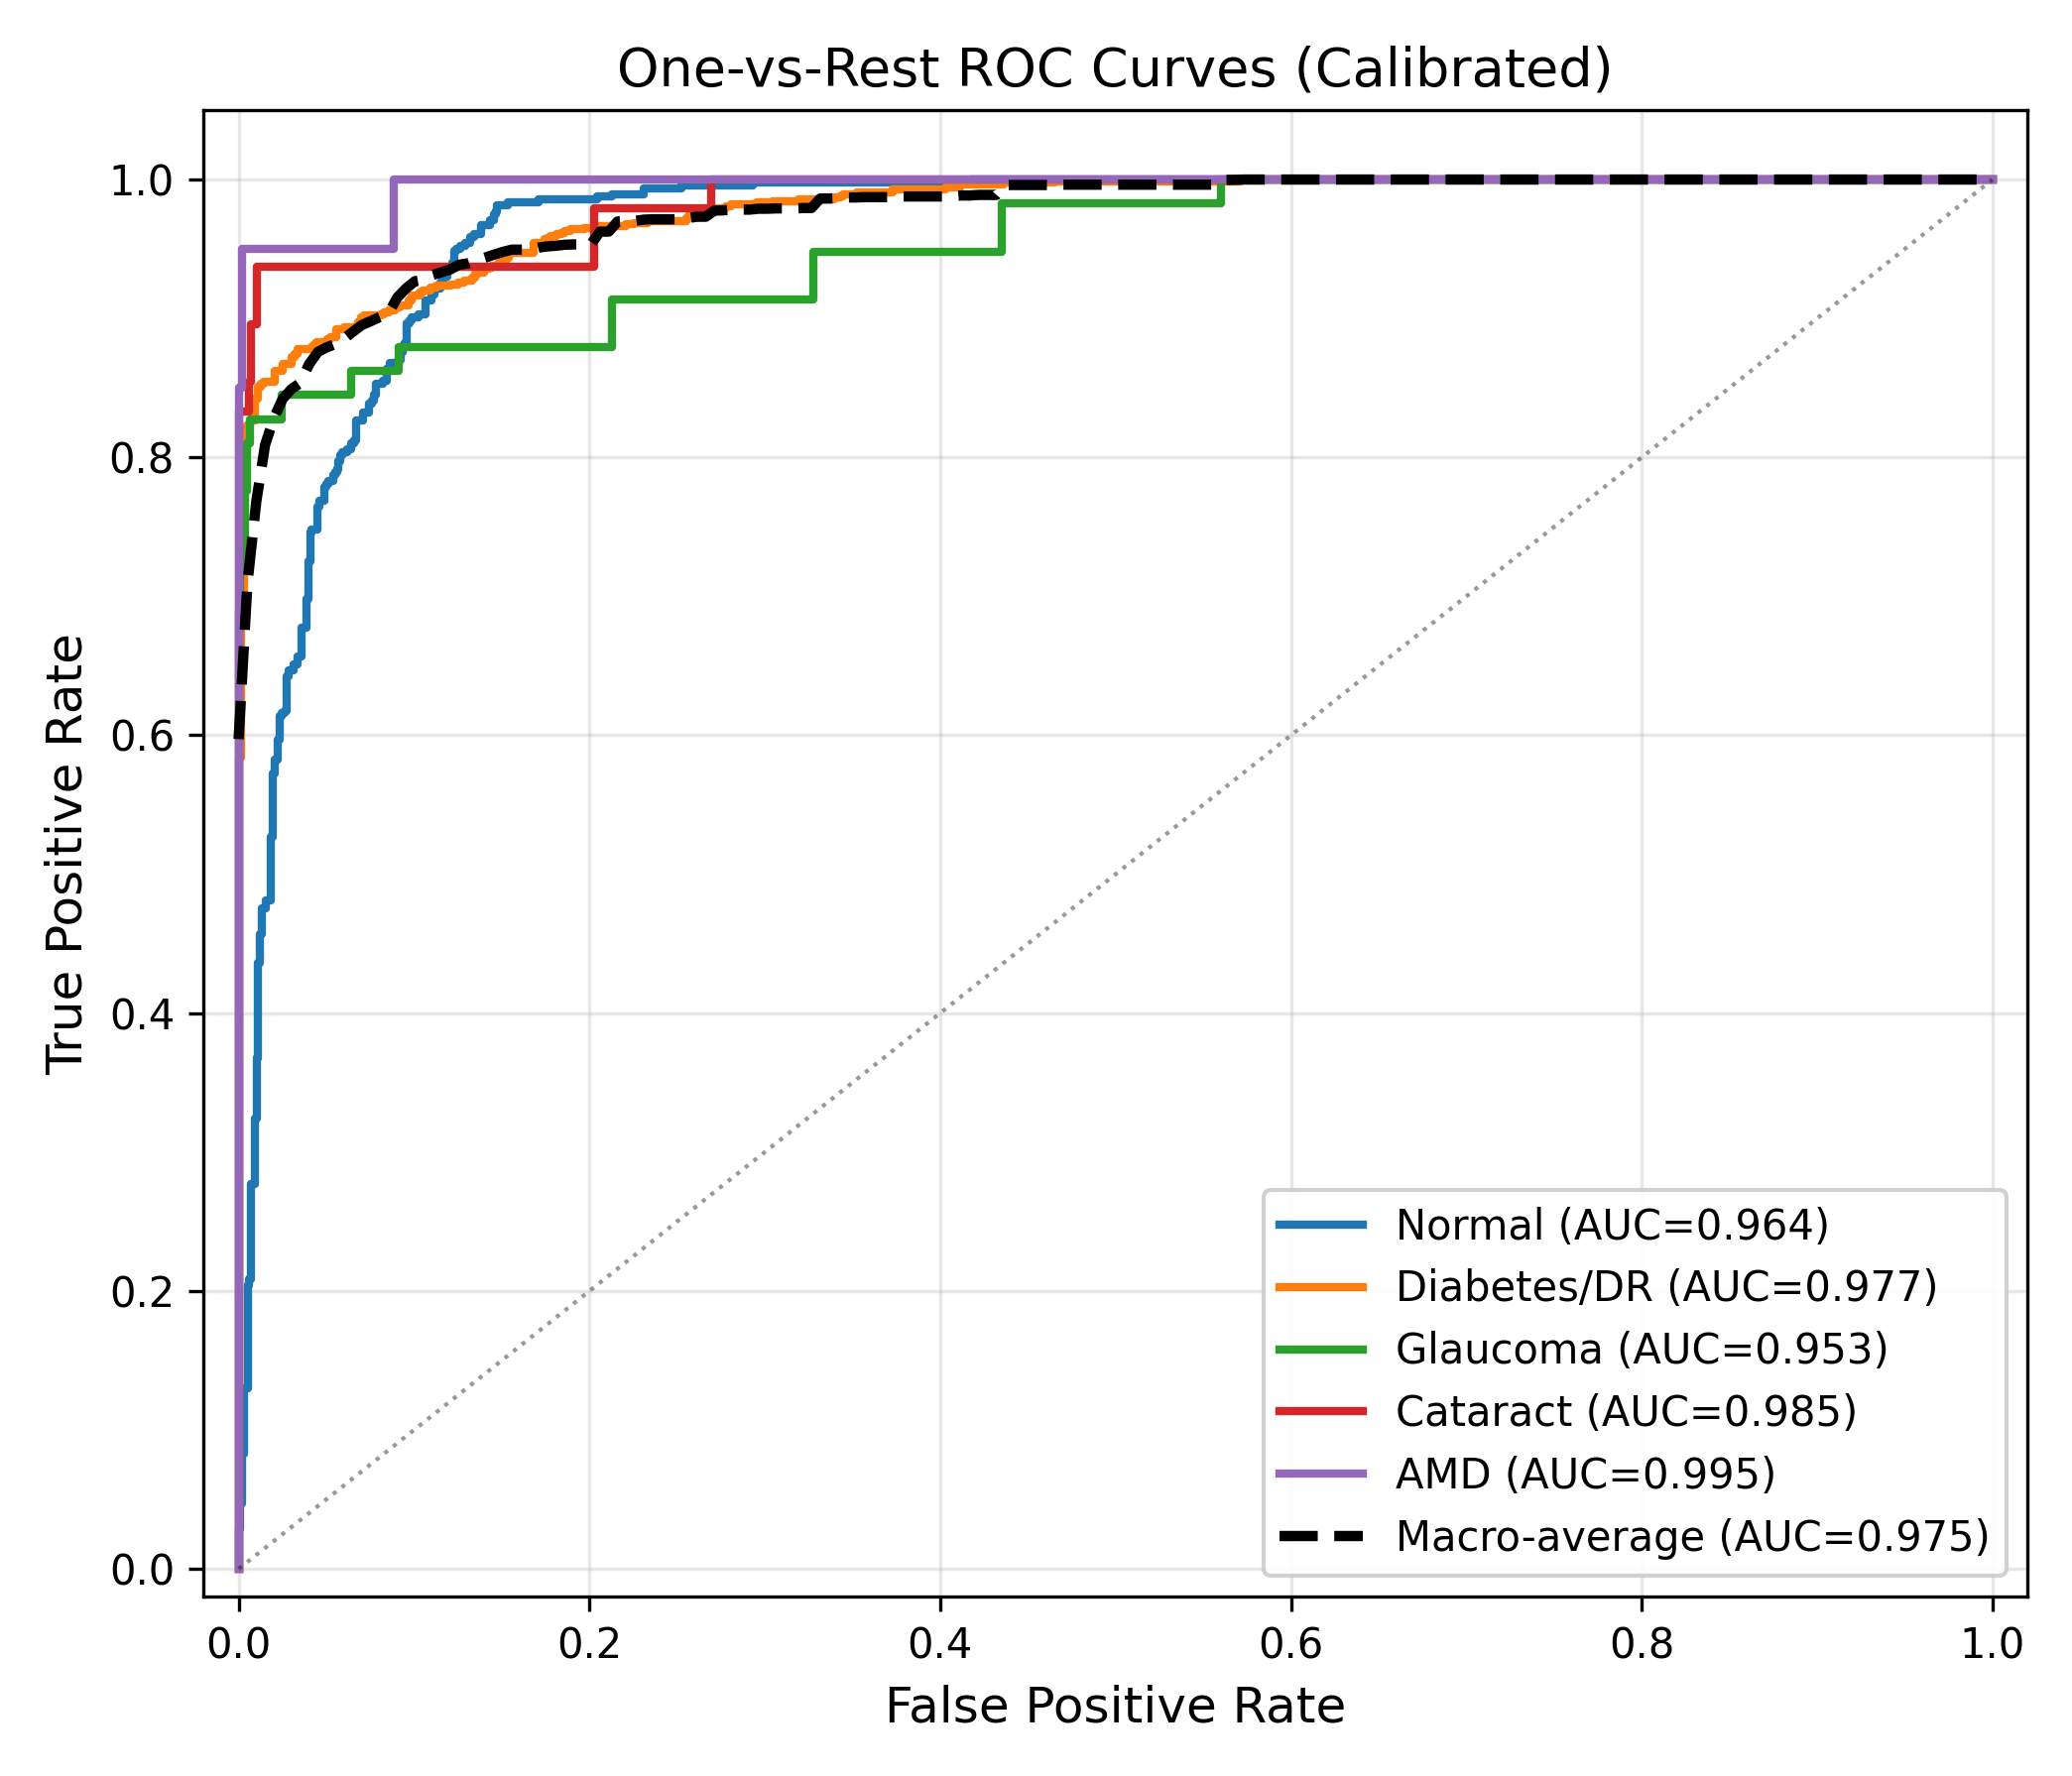
\includegraphics[width=0.95\linewidth]{figures/fig_roc_curves.png}
\caption{Per-class ROC curves on the test set. All five classes achieve AUC $>$ 0.95, with AMD reaching 0.995 despite having only 40 test samples.}
\label{fig:roc}
\end{figure}

\subsection{Domain Adaptation Effectiveness}

\begin{table}[h]
\centering
\caption{Per-Source Test Accuracy}
\label{tab:domain_acc}
\begin{tabular}{lrrl}
\toprule
\textbf{Source} & \textbf{Accuracy} & \textbf{$n$} & \textbf{Classes Present} \\
\midrule
APTOS & 100.0\% & 570 & DR only \\
REFUGE2 & 98.4\% & 188 & Normal, Glaucoma \\
ODIR & 78.1\% & 709 & All 5 classes \\
\bottomrule
\end{tabular}
\end{table}

\noindent Before DANN training, APTOS accuracy was only 26.5\%. The cause was preprocessing-induced domain shift: APTOS images turned out to be 10.7$\times$ sharper than those from ODIR. Switching to unified CLAHE preprocessing and adding DANN training eliminated this gap entirely.

\subsection{Calibration Analysis}

Temperature scaling with $T=0.566$ reduces the Expected Calibration Error from 0.150 to 0.034---a 77\% reduction. The reliability diagram in Fig.~\ref{fig:calibration} confirms that calibrated predictions track the ideal diagonal closely, which is what we need for the downstream confidence routing to work reliably.

\begin{figure}[h]
\centering
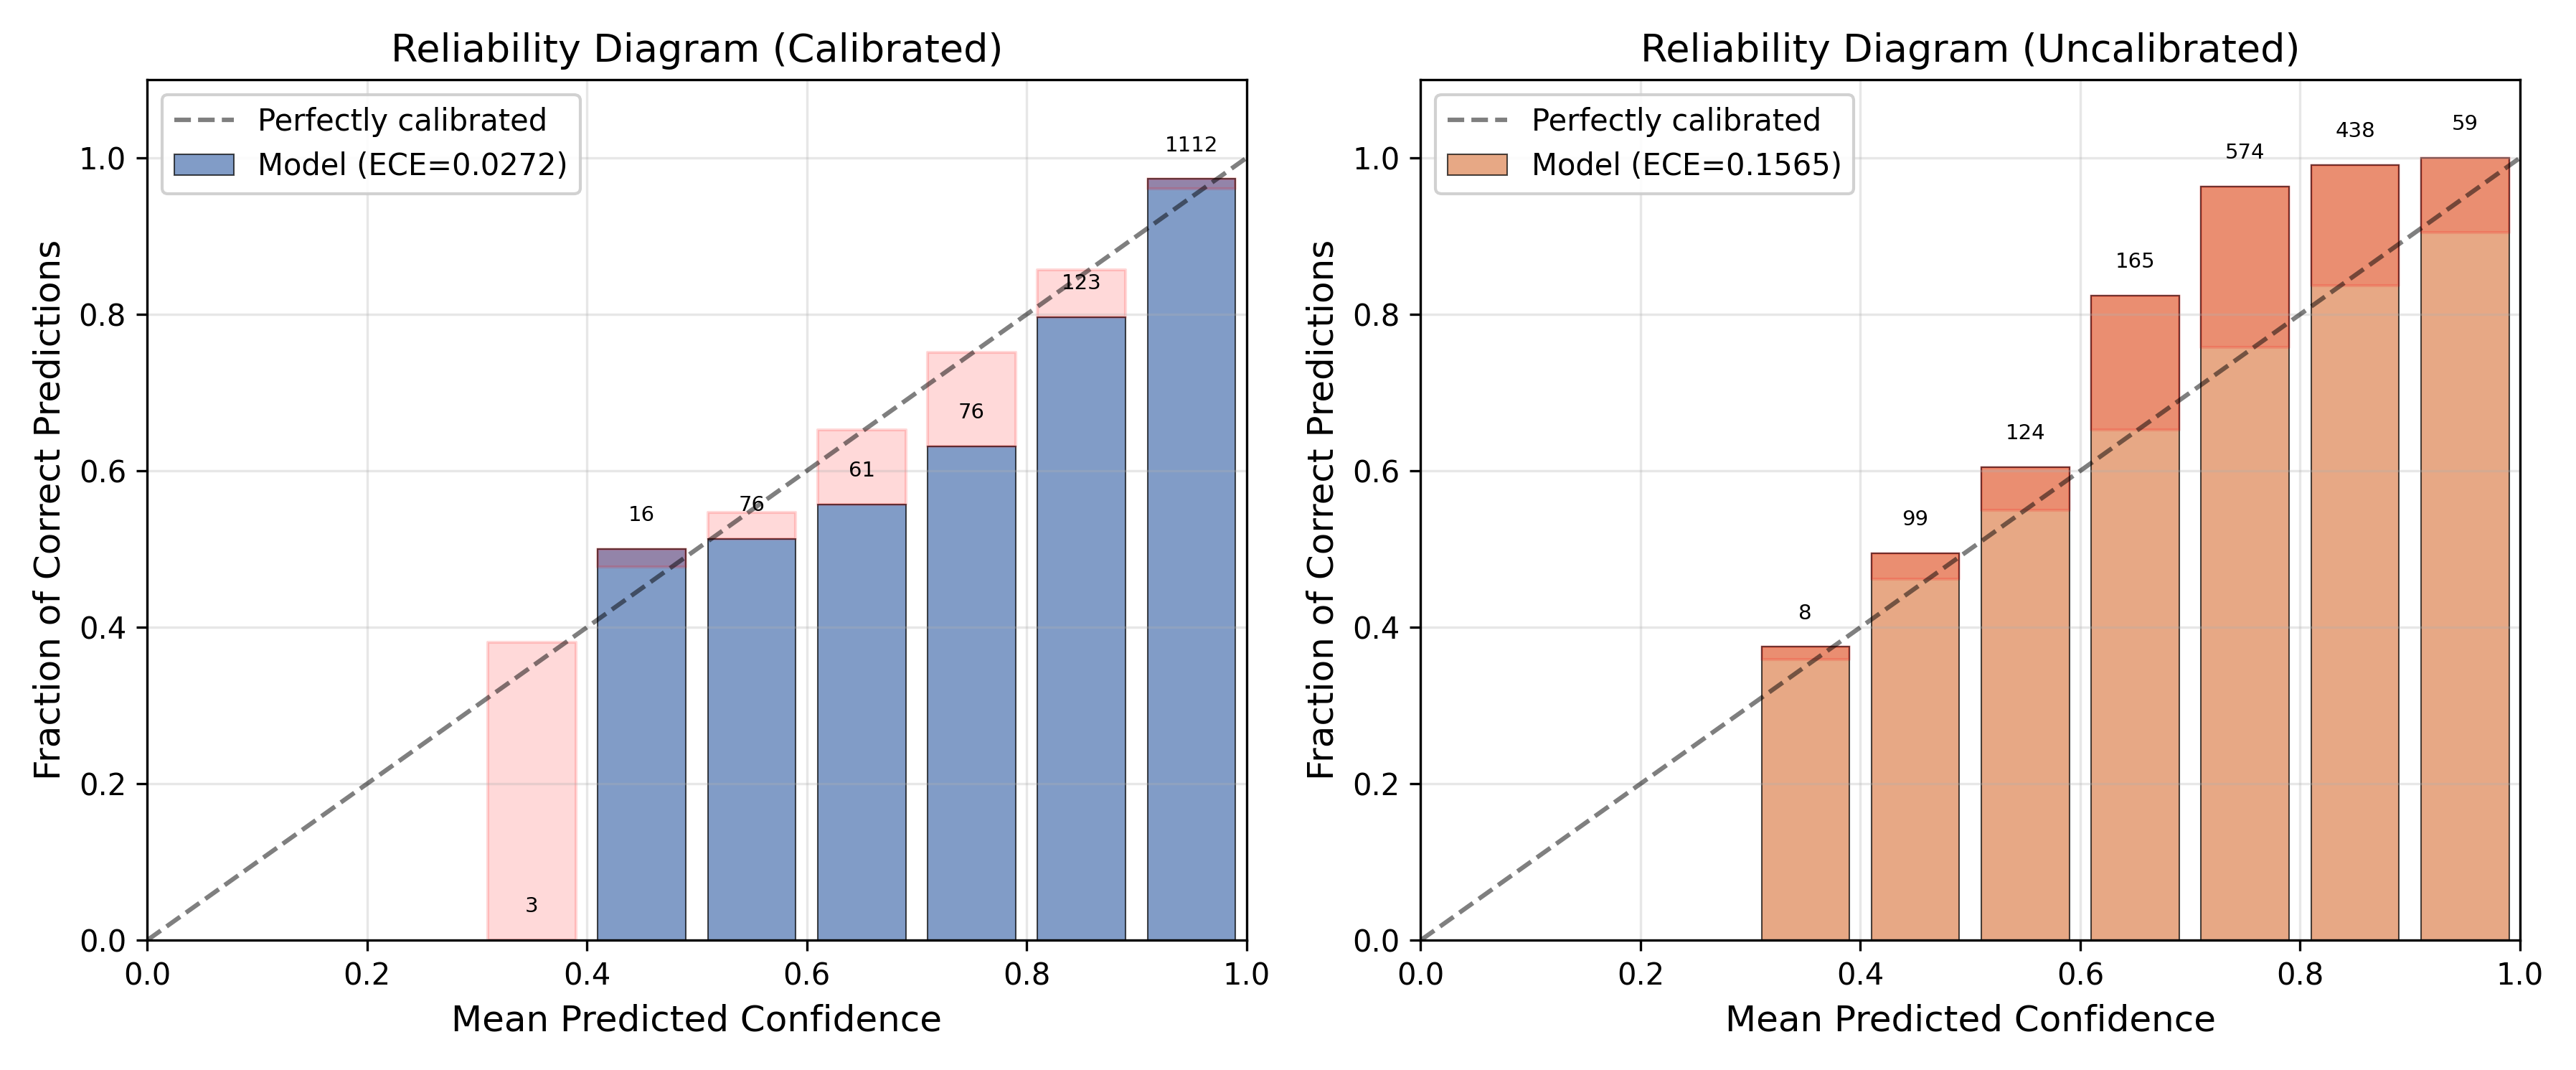
\includegraphics[width=0.95\linewidth]{figures/fig_calibration_reliability.png}
\caption{Reliability diagram showing calibrated (left) vs.\ uncalibrated (right) predictions. ECE reduces from 0.150 to 0.034 after temperature scaling.}
\label{fig:calibration}
\end{figure}

\subsection{Confusion Matrix and Error Analysis}

\begin{table}[h]
\centering
\caption{Test Set Confusion Matrix}
\label{tab:confusion}
\begin{tabular}{l|rrrrr}
\toprule
& \textbf{Nor} & \textbf{DR} & \textbf{Gla} & \textbf{Cat} & \textbf{AMD} \\
\midrule
\textbf{Normal} & \textbf{433} & 45 & 5 & 1 & 0 \\
\textbf{DR} & 78 & \textbf{757} & 0 & 0 & 2 \\
\textbf{Glaucoma} & 8 & 5 & \textbf{45} & 0 & 0 \\
\textbf{Cataract} & 8 & 0 & 0 & \textbf{40} & 0 \\
\textbf{AMD} & 3 & 3 & 0 & 0 & \textbf{34} \\
\bottomrule
\end{tabular}
\end{table}

\noindent The model makes 158 errors in total (10.7\% error rate), and 77\% of those involve confusion between Normal and DR: 78 cases where DR is called Normal (49\% of errors) and 45 where Normal is called DR (28\%). This is not surprising---early-stage DR can look nearly indistinguishable from a healthy fundus, even to experienced clinicians. Fig.~\ref{fig:cm} visualizes the full confusion pattern.

\begin{figure}[h]
\centering
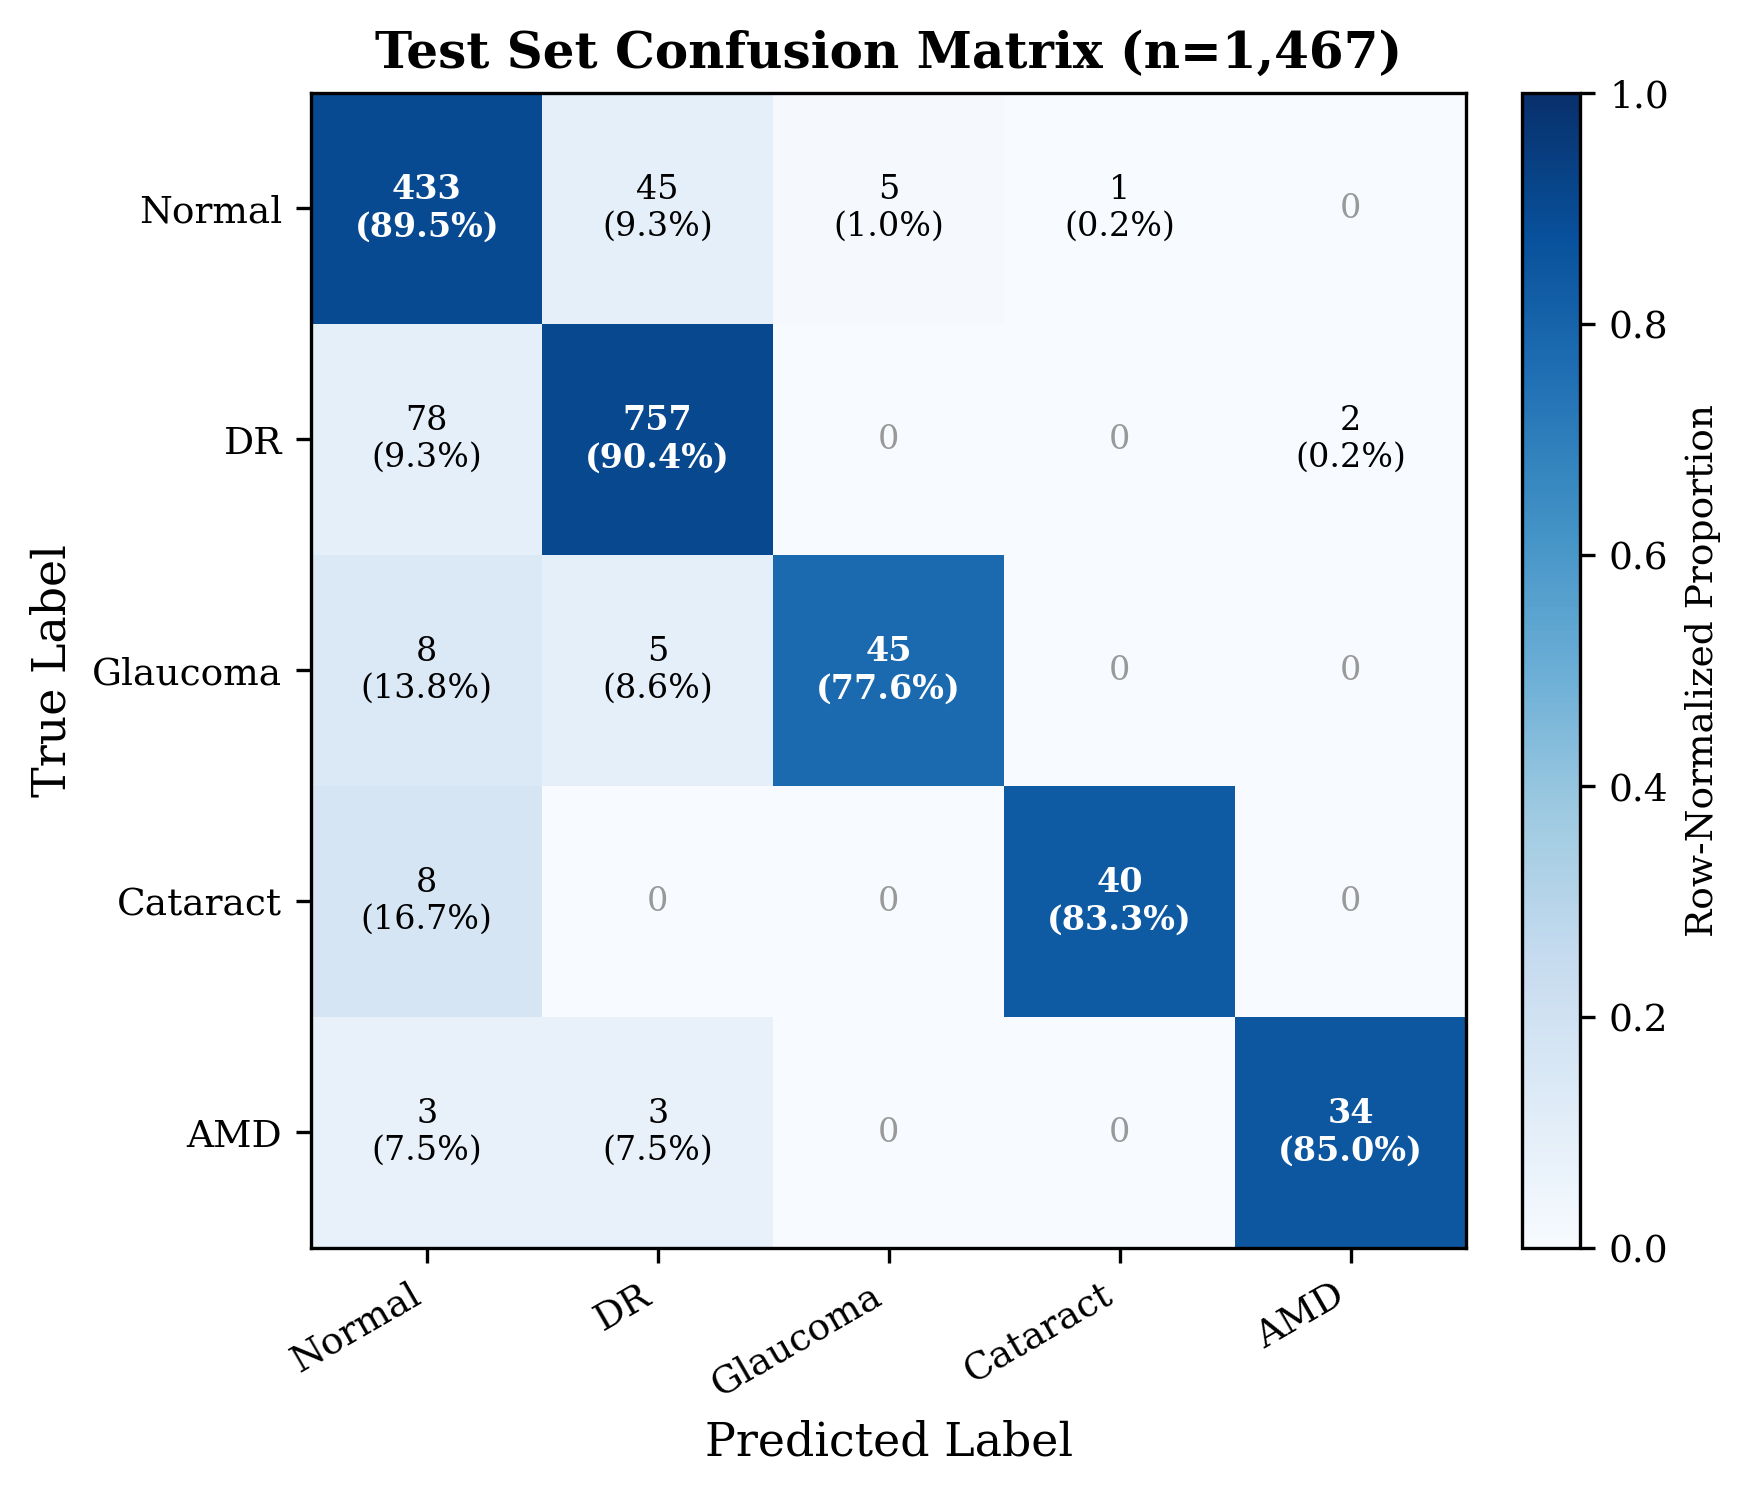
\includegraphics[width=0.75\linewidth]{figures/fig_confusion_matrix.png}
\caption{Row-normalized confusion matrix on the test set (n=1,467). Diagonal entries show correct classifications; off-diagonal entries reveal that Normal$\leftrightarrow$DR confusion accounts for 77\% of all errors.}
\label{fig:cm}
\end{figure}

\subsection{Retrieval-Augmented Diagnosis Results}

Our FAISS index holds 8,241 L2-normalized 768-dim ViT embeddings spanning all five classes. Table~\ref{tab:retrieval} reports retrieval quality on the test set.

\begin{table}[h]
\centering
\caption{Retrieval Quality Metrics (MAP = 0.921)}
\label{tab:retrieval}
\begin{tabular}{lrrrr}
\toprule
\textbf{Metric} & \textbf{K=1} & \textbf{K=3} & \textbf{K=5} & \textbf{K=10} \\
\midrule
Recall@K & 0.940 & 0.950 & 0.958 & 0.967 \\
Precision@K & 0.940 & 0.899 & 0.890 & 0.884 \\
Agreement Rate & 0.930 & 0.947 & 0.947 & 0.962 \\
kNN Accuracy & 0.940 & 0.898 & 0.903 & 0.901 \\
RAD Combined & 0.940 & 0.900 & 0.895 & 0.891 \\
\bottomrule
\end{tabular}
\end{table}

\noindent At $K\!=\!1$, the retrieved nearest neighbor matches the correct class 94.0\% of the time, and blending retrieval with the model's prediction pushes accuracy to 94.0\%---a $+4.9\%$ improvement over the standalone model (89.1\%). Per-class average precision follows an expected pattern: DR (0.952) and Normal (0.906) benefit from larger representation, while Cataract (0.833), AMD (0.819), and Glaucoma (0.742) reflect their smaller index populations. The consistently high agreement rate ($>$93\%) confirms that the learned embeddings capture real clinical similarity.

Per-source retrieval quality tracks domain complexity (Fig.~\ref{fig:recall_at_k}). APTOS achieves perfect recall (1.000 at every $K$), REFUGE2 is close behind at 0.984 ($K\!=\!1$), and ODIR---the most heterogeneous source, containing all five classes---reaches 0.879 ($K\!=\!1$), rising to 0.932 by $K\!=\!10$. That this source-level pattern mirrors the classification results suggests the retrieval difficulty stems from clinical complexity, not from indexing artifacts.

\begin{figure}[h]
\centering
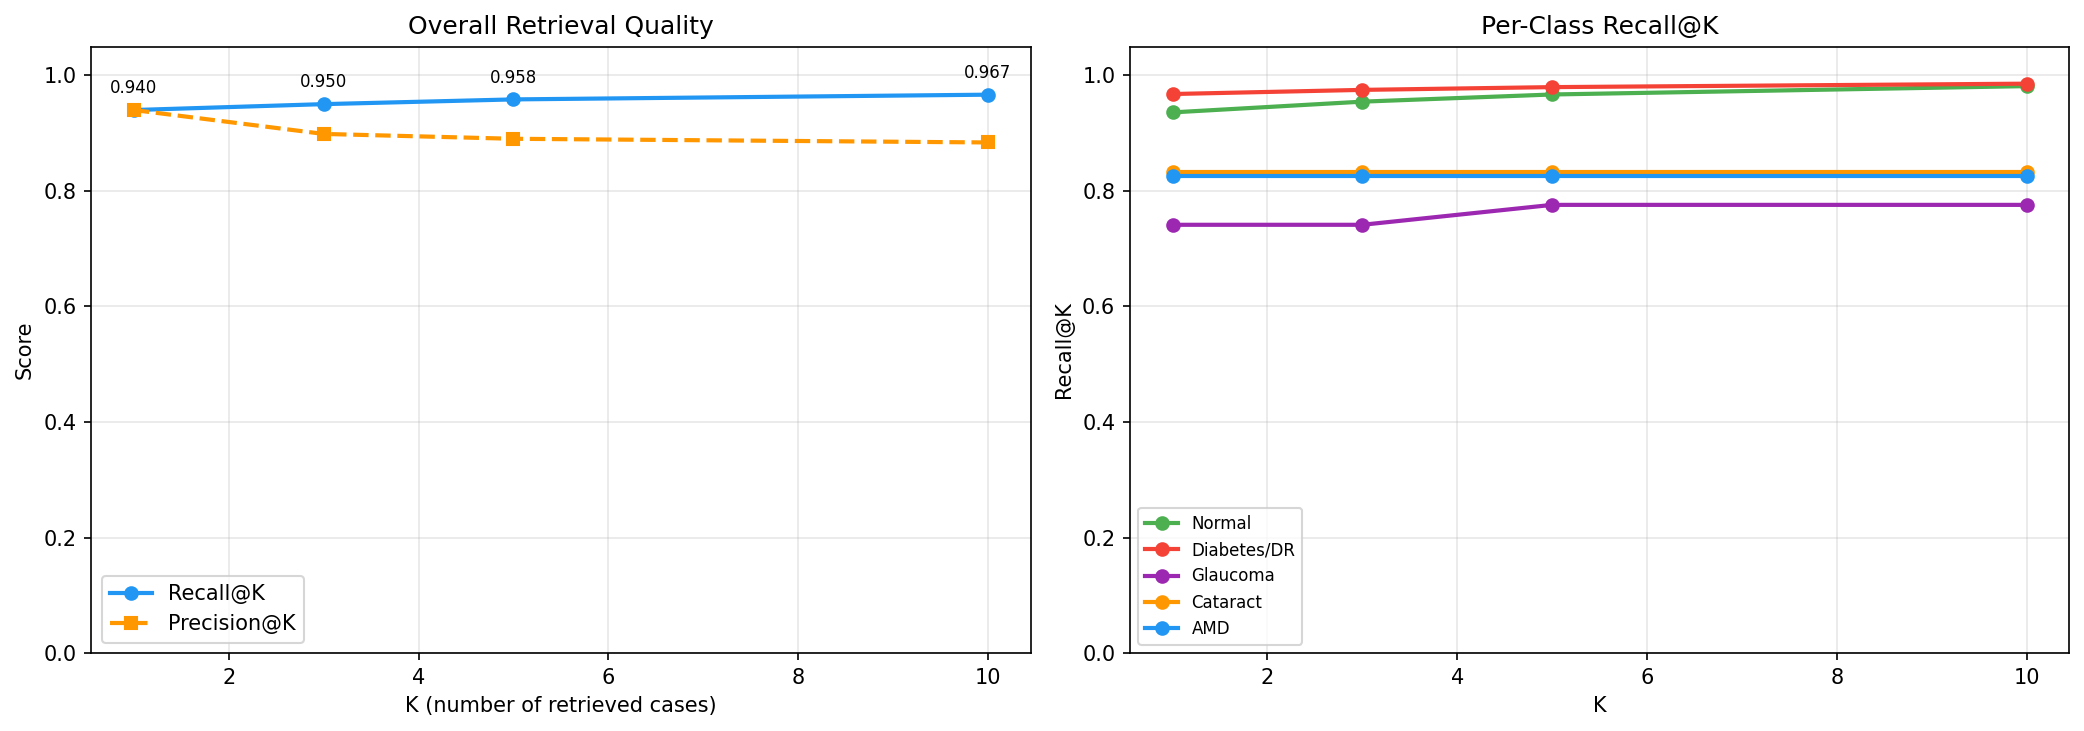
\includegraphics[width=0.95\linewidth]{figures/fig_retrieval_recall_at_k.png}
\caption{Retrieval Recall@K across different values of K, broken down by disease class. DR and Normal achieve highest recall due to larger training representation.}
\label{fig:recall_at_k}
\end{figure}

\subsection{Confidence Routing for Clinical Triage}

The confidence routing system assigns each test prediction to one of three tiers using model confidence, MC Dropout entropy ($T\!=\!15$ passes), and retrieval agreement ($K\!=\!5$):

\begin{table}[h]
\centering
\caption{Confidence Routing Tier Performance}
\label{tab:routing}
\begin{tabular}{lrrr}
\toprule
\textbf{Tier} & \textbf{Samples} & \textbf{\%} & \textbf{Accuracy} \\
\midrule
Auto-Report & 1,128 & 76.9\% & \textbf{96.8\%} \\
Review & 314 & 21.4\% & 65.6\% \\
Escalate & 25 & 1.7\% & 44.0\% \\
\bottomrule
\end{tabular}
\end{table}

\noindent In practice, this means roughly three-quarters of cases can be processed automatically at near-perfect accuracy (96.8\%), while 77.2\% of the model's errors (122 out of 158) get caught and redirected to human review before reaching the auto-report tier. Only 1.7\% of cases require specialist escalation. From a workflow perspective, a screening center could potentially handle around $4\times$ the volume if an ophthalmologist only needs to review the 23.1\% of cases that are not auto-reported. Fig.~\ref{fig:routing} breaks down the routing by tier and class.

\begin{figure}[h]
\centering
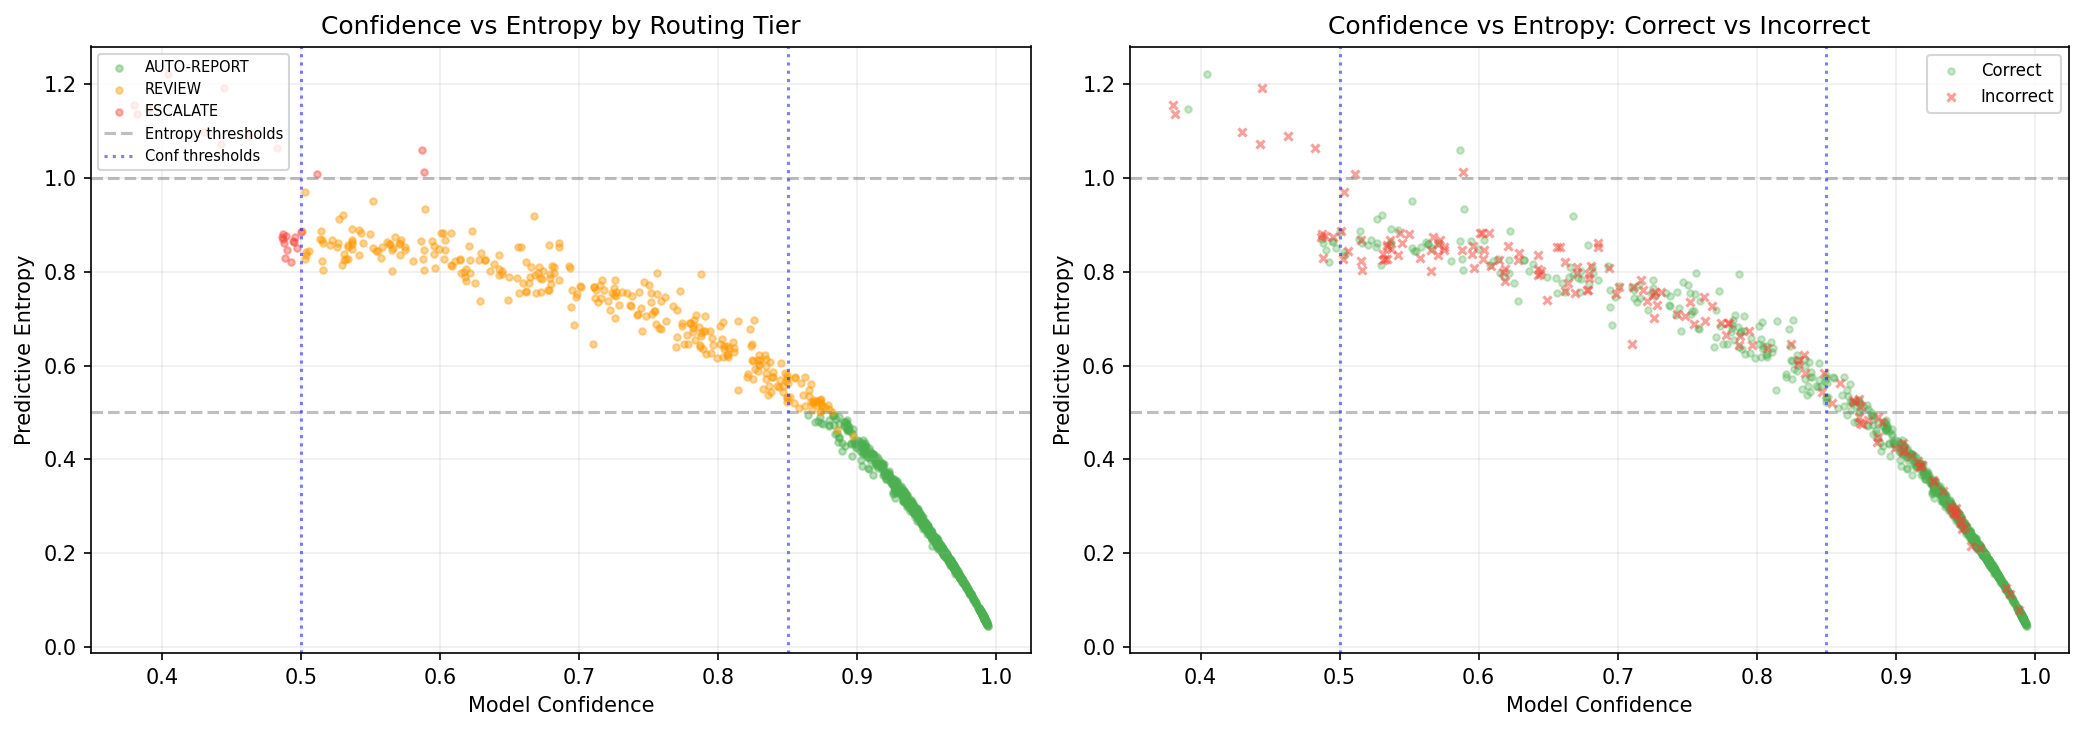
\includegraphics[width=0.95\linewidth]{figures/fig_routing_analysis.png}
\caption{Confidence routing analysis: tier distribution, per-tier accuracy, and per-class routing breakdown. Auto-report tier achieves 96.8\% accuracy on 76.9\% of cases.}
\label{fig:routing}
\end{figure}

% ================================================================
% VII. ABLATION STUDY
% ================================================================
\section{Ablation Study}

\subsection{Model Architecture and Training Progression}

To isolate the contribution of each component, we ran a controlled ablation where every variant was trained from scratch for 20 epochs on an H100 GPU. Results appear in Table~\ref{tab:ablation}. (The full pipeline scores 89.09\% here, slightly below the 89.30\% of the final model, because the final model trained for 40 epochs and benefited from warm-starting.)

\begin{table}[h]
\centering
\caption{Controlled Ablation Study (GPU-Trained, 20 epochs each). Note: the full pipeline achieves 89.09\% here (20 epochs from scratch) vs.\ 89.30\% for the final model (40 epochs, warm-started).}
\label{tab:ablation}
\begin{tabular}{lcccc}
\toprule
\textbf{Model Variant} & \textbf{Acc} & \textbf{F1} & \textbf{AUC} & \textbf{ECE} \\
\midrule
Base ViT (no DANN) & 85.28\% & 0.843 & 0.944 & 0.051 \\
DANN only & 84.73\% & 0.843 & 0.937 & 0.078 \\
DANN + hard mining & 85.89\% & 0.849 & 0.947 & 0.087 \\
DANN + mixup & 84.66\% & 0.821 & 0.931 & 0.131 \\
\textbf{DANN-v3 (full pipeline)} & \textbf{89.09\%} & \textbf{0.879} & \textbf{0.972} & 0.157 \\
\bottomrule
\end{tabular}
\end{table}

\begin{figure}[h]
\centering
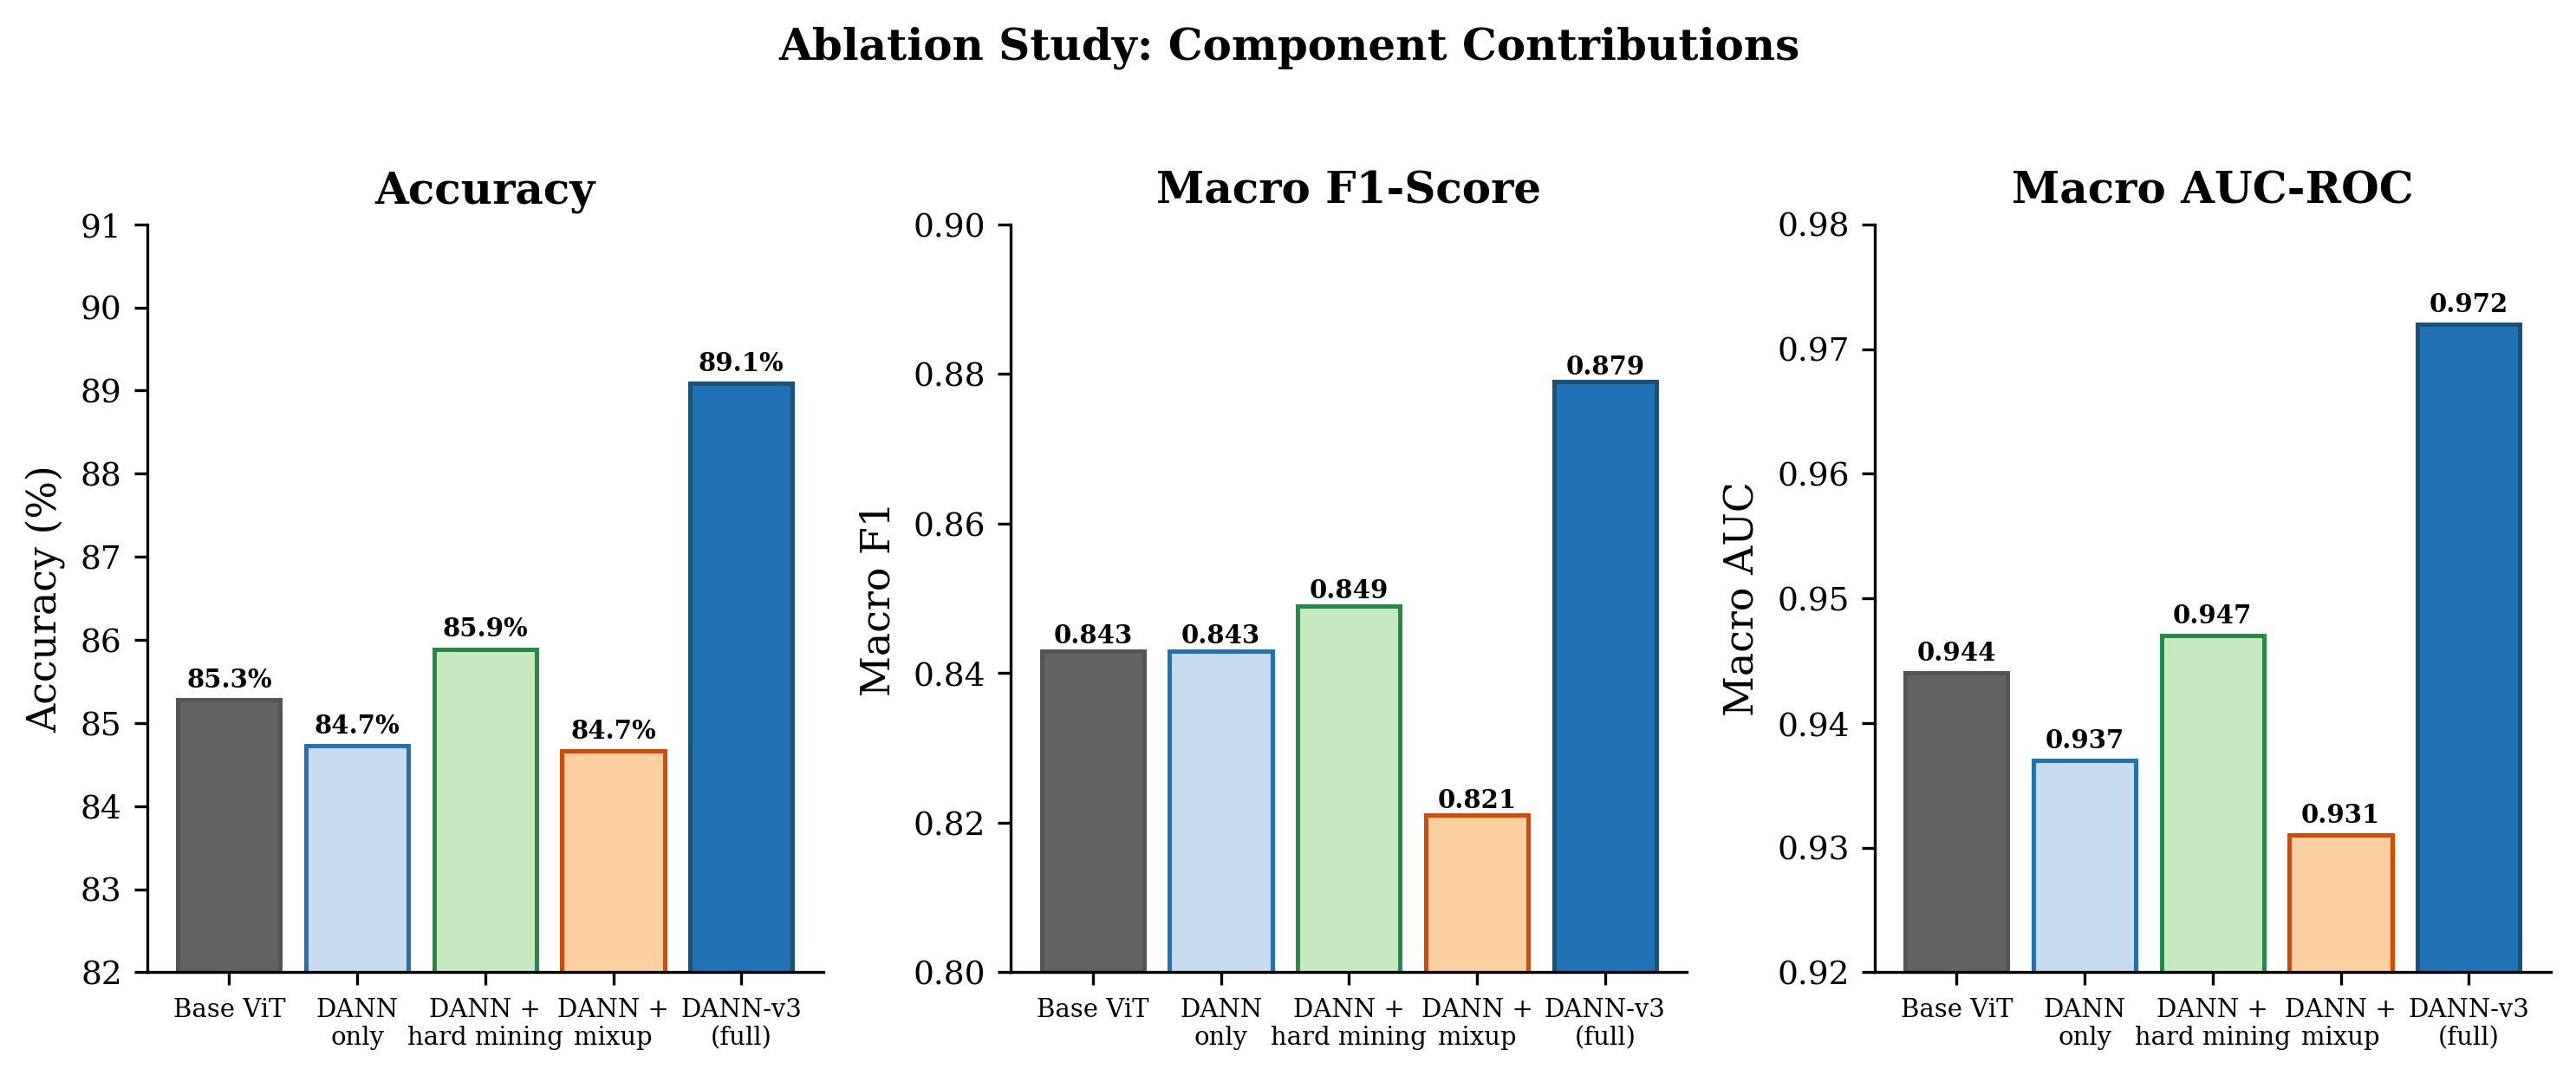
\includegraphics[width=0.95\linewidth]{figures/fig_ablation.png}
\caption{Ablation study comparing accuracy, macro F1, and macro AUC across model variants. The full DANN-v3 pipeline achieves the best performance across all three metrics, demonstrating the synergy of all training components.}
\label{fig:ablation}
\end{figure}

\subsection{Impact of Individual Components}

The pattern in Fig.~\ref{fig:ablation} is clear. The full pipeline outperforms the base ViT by $+3.82\%$ in accuracy, but no single component accounts for this gain on its own. DANN alone actually hurts slightly ($-0.55\%$), which tells us that learning domain-invariant features is not enough without the other training strategies to complement it. Hard-example mining contributes the largest single improvement ($+0.61\%$), largely by targeting the DR$\rightarrow$Normal misclassification mode and cutting it from 154 to 78 cases. Mixup in isolation also degrades performance ($-0.61\%$), yet it clearly helps when combined with the remaining strategies. The key observation is that the eight strategies are synergistic---the combined effect exceeds what you would get by adding up their individual contributions. The full pipeline's pre-calibration ECE of 0.157 drops to 0.034 after temperature scaling.

\subsection{Impact of Threshold Optimization}

Optimizing per-class decision thresholds on the calibration set adds $+2.22\%$ accuracy over raw argmax predictions, and it costs nothing at inference time. The optimized thresholds are particularly useful for minority classes: AMD's threshold drops to 0.344 and Cataract's to 0.289, making the model more willing to predict these rare conditions, while Glaucoma's threshold stays relatively high at 0.674.

\subsection{Cross-Validation Results}

We ran five-fold stratified cross-validation on the combined train and calibration pool (10,057 images) to gauge stability:

\begin{table}[h]
\centering
\caption{5-Fold Cross-Validation Results}
\label{tab:kfold}
\begin{tabular}{lc}
\toprule
\textbf{Metric} & \textbf{Mean $\pm$ Std} \\
\midrule
Accuracy & 82.4\% $\pm$ 1.9\% \\
Macro F1 & 0.827 $\pm$ 0.019 \\
Macro AUC & 0.948 $\pm$ 0.008 \\
\bottomrule
\end{tabular}
\end{table}

\noindent The low fold-to-fold variance confirms stable learning. The gap between k-fold performance (82.4\%) and the final model (89.3\%) is expected: the k-fold experiment did not include DANN domain adaptation or the MESSIDOR-2 data that was added later.

\subsection{Leave-One-Domain-Out (LODO) Validation}

As a more stringent test of generalization, we train on three of the four domains and evaluate on the held-out domain:

\begin{table}[h]
\centering
\caption{Leave-One-Domain-Out (LODO) Validation}
\label{tab:lodo}
\begin{tabular}{lccccr}
\toprule
\textbf{Held-Out} & \textbf{Acc} & \textbf{wF1} & \textbf{Classes} & \textbf{$n$} \\
\midrule
APTOS & 70.8\% & 0.829 & DR only & 3,662 \\
MESSIDOR-2 & 61.6\% & 0.633 & Nor, DR & 1,744 \\
ODIR & 51.8\% & 0.439 & All 5 & 4,878 \\
REFUGE2 & \textbf{88.8\%} & \textbf{0.904} & Nor, Gla & 1,240 \\
\midrule
\textbf{Average} & \textbf{68.2\%} & 0.701 & --- & --- \\
\bottomrule
\end{tabular}
\end{table}

\noindent These results reveal interesting domain-specific patterns. REFUGE2 transfers best (88.8\%), suggesting that Normal vs. Glaucoma discrimination generalizes well across sources. APTOS reaches a respectable 70.8\% for DR detection without ever seeing APTOS images during training. ODIR proves the hardest to generalize to (51.8\%), which makes sense: it is the only source containing all five classes, so holding it out means the training set has no Cataract or AMD examples at all. Even so, the model still manages 65.1\% F1 on Normal and 39.6\% on DR for ODIR images it was never trained on.

% ================================================================
% VIII. COMPARISON WITH EXISTING WORK
% ================================================================
\section{Comparison with Existing Work}

Table~\ref{tab:sota} puts our results alongside published methods. Direct comparison is not straightforward because we are tackling a harder problem---five-class classification across four heterogeneous sources with 21:1 class imbalance and a full clinical pipeline---but the numbers are encouraging.

\vspace{0.5em}
\noindent
\begin{minipage}{\linewidth}
\centering
\captionof{table}{Comparison with Published Methods}
\label{tab:sota}
\small
\begin{tabular}{lccp{1.6cm}}
\toprule
\textbf{Method} & \textbf{Acc} & \textbf{AUC} & \textbf{Task} \\
\midrule
Gulshan \cite{b3} & -- & 0.991 & DR binary \\
RETFound \cite{b22} & -- & 0.822--0.978 & Various \\
DKCNet \cite{b23} & -- & 0.961 & ODIR 8-cls \\
Ahmed \cite{b24} & 84.6\% & -- & DR 5-class \\
Wang \cite{b14} & 87.2\% & 0.965 & Multi-dis. \\
\midrule
\textbf{Ours} & \textbf{89.3\%} & \textbf{0.975} & \textbf{Multi-dis. 4 src + RAD} \\
\bottomrule
\end{tabular}
\end{minipage}
\vspace{0.5em}

% ================================================================
% IX. DISCUSSION
% ================================================================
\section{Discussion}

\subsection{Clinical Implications}

One of the biggest barriers to deploying AI in the clinic is trust, and the RAD pipeline is designed to address this directly. Instead of handing the clinician a single label, RetinaSense provides calibrated confidence, uncertainty estimates, attention maps highlighting the regions the model focused on, and a set of similar historical cases. The idea is to let the clinician \textit{verify} the prediction rather than accept it blindly.

The confidence routing system is where this becomes practical at scale. With 76.9\% of predictions going straight to auto-report at 96.8\% accuracy---and 77.2\% of errors caught before they reach that tier---an ophthalmologist would only need to review about 23\% of cases. In a screening center with limited specialists, that could translate to roughly a $4\times$ increase in throughput.

\subsection{Domain Adaptation Impact}

The DANN component addresses what was, for us, a critical practical problem: how to combine datasets from different sources without having to hand-tune for each one. The Gradient Reversal Layer pushes the backbone to ignore source-specific artifacts---such as camera-specific color profiles or resolution differences---and focus on features that are diagnostically relevant across all sources. The most dramatic example is APTOS, where accuracy jumped from 26.5\% to 100\% once we moved to unified CLAHE preprocessing combined with adversarial training.

\subsection{Limitations}

Several limitations should be acknowledged. Our test set is drawn from the same four sources as the training data, so while the model handles cross-source variation within these datasets, we cannot make strong claims about generalization to entirely new populations or camera systems without external validation. The minority class test sets are also quite small (40--58 samples), which limits the statistical power of per-class comparisons. And we have not yet tested the system in a prospective clinical setting with ophthalmologists, which remains an important next step.

% ================================================================
% X. CONCLUSION
% ================================================================
\section{Conclusion}

We have presented RetinaSense, a framework for multi-disease retinal screening that integrates domain-adversarial training, calibrated uncertainty estimation, and retrieval-augmented reasoning into a unified clinical pipeline. Across five retinal conditions and four data sources, the system achieves 89.30\% accuracy, 0.886 macro F1, and 0.975 macro AUC, while giving clinicians interpretable evidence alongside each prediction.

Three findings stand out from our experiments. First, the full DANN-ViT pipeline gains $+3.82\%$ in accuracy over the base ViT (from 85.28\% to 89.09\%) in a controlled ablation, with domain adaptation and the progressive training strategies working together rather than any single technique being responsible. Second, the combination of eight training strategies proves essential for handling simultaneous domain shift and 21:1 class imbalance---no single strategy is sufficient on its own. Third, and perhaps most practically relevant, the RAD pipeline turns the classifier into something closer to a clinical decision-support tool: retrieval augmentation lifts accuracy from 89.3\% to 94.0\% at $K\!=\!1$, and confidence routing auto-reports 76.9\% of cases at 96.8\% accuracy while catching 77.2\% of errors.

Going forward, we plan to validate on external clinical datasets that the model has never seen, explore a RETFound backbone for domain-specific pre-training, investigate knowledge distillation for deployment on edge devices, and ultimately run a prospective evaluation with practicing ophthalmologists.

% ================================================================
% REFERENCES
% ================================================================
\begin{thebibliography}{00}

\bibitem{b1}
World Health Organization, ``World Report on Vision,'' 2019.

\bibitem{b2}
S. Resnikoff \textit{et al.}, ``Global data on visual impairment in the year 2002,'' \textit{Bull. World Health Org.}, vol. 82, no. 11, pp. 844--851, 2004.

\bibitem{b3}
V. Gulshan \textit{et al.}, ``Development and validation of a deep learning algorithm for detection of diabetic retinopathy,'' \textit{JAMA}, vol. 316, no. 22, pp. 2402--2410, 2016.

\bibitem{b4}
R. Poplin \textit{et al.}, ``Prediction of cardiovascular risk factors from retinal fundus photographs via deep learning,'' \textit{Nature Biomed. Eng.}, vol. 2, pp. 158--164, 2018.

\bibitem{b5}
M. Tan and Q. V. Le, ``EfficientNet: Rethinking model scaling for convolutional neural networks,'' in \textit{Proc. ICML}, 2019, pp. 6105--6114.

\bibitem{b6}
K. He \textit{et al.}, ``Deep residual learning for image recognition,'' in \textit{Proc. IEEE CVPR}, 2016, pp. 770--778.

\bibitem{b7}
Y. Gal and Z. Ghahramani, ``Dropout as a Bayesian approximation: Representing model uncertainty in deep learning,'' in \textit{Proc. ICML}, 2016.

\bibitem{b8}
A. Dosovitskiy \textit{et al.}, ``An image is worth 16x16 words: Transformers for image recognition at scale,'' in \textit{Proc. ICLR}, 2021.

\bibitem{b9}
J. Johnson, M. Douze, and H. J\'{e}gou, ``Billion-scale similarity search with GPUs,'' \textit{IEEE Trans. Big Data}, vol. 7, no. 3, pp. 535--547, 2021.

\bibitem{b10}
R. R. Selvaraju \textit{et al.}, ``Grad-CAM: Visual explanations from deep networks via gradient-based localization,'' in \textit{Proc. IEEE ICCV}, 2017, pp. 618--626.

\bibitem{b11}
H. Zhang \textit{et al.}, ``mixup: Beyond empirical risk minimization,'' in \textit{Proc. ICLR}, 2018.

\bibitem{b12}
T.-Y. Lin \textit{et al.}, ``Focal loss for dense object detection,'' in \textit{Proc. IEEE ICCV}, 2017, pp. 2980--2988.

\bibitem{b13}
Y. Ganin \textit{et al.}, ``Domain-adversarial training of neural networks,'' \textit{J. Machine Learning Research}, vol. 17, no. 59, pp. 1--35, 2016.

\bibitem{b14}
S. Wang \textit{et al.}, ``Benchmarking deep learning models for retinal disease classification,'' \textit{IEEE Access}, vol. 9, pp. 148026--148038, 2021.

\bibitem{b15}
J. Chen \textit{et al.}, ``TransUNet: Transformers make strong encoders for medical image segmentation,'' \textit{arXiv:2102.04306}, 2021.

\bibitem{b16}
Q. Dou \textit{et al.}, ``PnP-AdaNet: Plug-and-play adversarial domain adaptation network at unpaired cross-modality cardiac segmentation,'' \textit{IEEE Access}, vol. 7, pp. 99065--99076, 2019.

\bibitem{b17}
S. Abnar and W. Zuidema, ``Quantifying attention flow in transformers,'' in \textit{Proc. ACL}, 2020, pp. 4190--4197.

\bibitem{b18}
ODIR-5K, ``Peking University International Competition on Ocular Disease Intelligent Recognition,'' 2019. [Online]. Available: \url{https://odir2019.grand-challenge.org/}

\bibitem{b19}
APTOS 2019, ``Asia Pacific Tele-Ophthalmology Society Blindness Detection,'' [Online]. Available: \url{https://www.kaggle.com/c/aptos2019-blindness-detection}

\bibitem{b20}
REFUGE2 Challenge, ``Retinal Fundus Glaucoma Challenge Edition 2,'' 2020. [Online]. Available: \url{https://refuge.grand-challenge.org/}

\bibitem{b21}
E. Decenci\`{e}re \textit{et al.}, ``Feedback on a publicly distributed image database: The Messidor database,'' \textit{Image Analysis \& Stereology}, vol. 33, no. 3, pp. 231--234, 2014.

\bibitem{b22}
Y. Zhou \textit{et al.}, ``A foundation model for generalizable disease detection from retinal images,'' \textit{Nature}, vol. 622, pp. 156--163, 2023.

\bibitem{b23}
N. Li \textit{et al.}, ``DKCNet: A dual-branch multi-label classification network for ocular disease detection,'' \textit{IEEE Trans. Instrum. Meas.}, vol. 72, 2023.

\bibitem{b24}
S. Ahmed \textit{et al.}, ``Automated detection of diabetic retinopathy using deep learning,'' \textit{Comp. Methods Programs Biomed.}, vol. 211, 106391, 2021.

\bibitem{b25}
D. P. Kingma and J. Ba, ``Adam: A method for stochastic optimization,'' in \textit{Proc. ICLR}, 2015.

\bibitem{b26}
M. Buda, A. Maki, and M. A. Mazurowski, ``A systematic study of the class imbalance problem in convolutional neural networks,'' \textit{Neural Netw.}, vol. 106, pp. 249--259, 2018.

\bibitem{b27}
F. Grassmann \textit{et al.}, ``A deep learning algorithm for prediction of AMD severity from color fundus photography,'' \textit{Ophthalmology}, vol. 125, no. 9, pp. 1410--1420, 2018.

\bibitem{b28}
H. Touvron \textit{et al.}, ``Training data-efficient image transformers \& distillation through attention,'' in \textit{Proc. ICML}, 2021, pp. 10347--10357.

\bibitem{b29}
B. Graham, ``Kaggle diabetic retinopathy detection competition report,'' 2015.

\bibitem{b30}
R. Wightman, ``PyTorch Image Models (timm),'' GitHub, 2019. [Online]. Available: \url{https://github.com/rwightman/pytorch-image-models}

\end{thebibliography}

\end{document}
